\documentclass [11pt,twoside]{article}
\usepackage[utf8]{inputenc}
\usepackage[T1]{fontenc}

%Page margins, header and footer positions
\usepackage{geometry}
 \geometry{
 a4paper,
 total={210mm,297mm},
 left=25mm,
 right=25mm,
 top=30mm,
 bottom=25mm,
 headsep=7mm}

\interfootnotelinepenalty=10000

%To display filling dots in the TOC for all entries
\usepackage[titles]{tocloft}
\renewcommand{\cftsecleader}{\cftdotfill{\cftdotsep}}

%Define new header and footer style
\usepackage{fancyhdr}

\pagestyle{fancy}
\fancyhf{}
\lhead{\color{Gray}{\small{Travlendar+ project by YOUR NAMES}}}
\lfoot{\textcolor{Gray}{\small{Copyright © 2017, YOUR NAMES – All rights reserved}}}
\rfoot{\textcolor{Gray}{\thepage}}
\renewcommand{\headrulewidth}{0pt}

%PACKAGES
\usepackage{wasysym}
\usepackage{pifont}

\newcommand{\supported}{\ding{52}\xspace}
\newcommand{\unsupported}{\ding{55}\xspace}
\newcommand{\partsupported}{\textcolor{black!40}{\ding{52}}\xspace}
\newcommand{\lowsupported}{\textcolor{black!20}{\ding{52}}\xspace}
\newcommand{\unknowsupported}{\textbf{?}\xspace}

%Font: Times
\usepackage{times}
%Change monospaced font
\renewcommand{\ttdefault}{lmtt}

%tables
\usepackage{tabu}
\usepackage{tabularx}
\usepackage{ltablex}
\usepackage{longtable}
\usepackage{float} % To allow the use of H modifier in long tables

%landscape mode
\usepackage{pdflscape}
\usepackage{rotating}
\usepackage{caption}

%make landscape mode be sensitive to even and odd pages
%start
\def\myrotate{\ifodd\c@page\else-\fi 90}
\makeatletter
\global\let\orig@begin@landscape=\landscape%
\global\let\orig@end@landscape=\endlandscape%
\gdef\@true{1}
\gdef\@false{0}
\gdef\landscape{%
    \global\let\within@landscape=\@true%
    \orig@begin@landscape%
}%
\gdef\endlandscape{%
    \orig@end@landscape%
    \global\let\within@landscape=\@false%
}%
\@ifpackageloaded{pdflscape}{%
    \gdef\pdf@landscape@rotate{\PLS@Rotate}%
}{
    \gdef\pdf@landscape@rotate#1{}%
}
\let\latex@outputpage\@outputpage
\def\@outputpage{
    \ifx\within@landscape\@true%
        \if@twoside%
            \ifodd\c@page%
                \gdef\LS@rot{\setbox\@outputbox\vbox{%
                    \pdf@landscape@rotate{-90}%
                    \hbox{\rotatebox{90}{\hbox{\rotatebox{180}{\box\@outputbox}}}}}%
                }%
            \else%
                \gdef\LS@rot{\setbox\@outputbox\vbox{%
                    \pdf@landscape@rotate{+90}%
                    \hbox{\rotatebox{90}{\hbox{\rotatebox{0}{\box\@outputbox}}}}}%
                }%
            \fi%
        \else%
            \gdef\LS@rot{\setbox\@outputbox\vbox{%
                \pdf@landscape@rotate{+90}%
                \hbox{\rotatebox{90}{\hbox{\rotatebox{0}{\box\@outputbox}}}}}%
            }%
        \fi%
    \fi%
    \latex@outputpage%
}
\makeatother
%end

%graphics
\usepackage{graphicx}
\usepackage[dvipsnames, table]{xcolor}
%If you upload images from PC, you need to insert code for the path here (different for Windows and Unix OS)

%References
%\usepackage{xpatch}
%\usepackage[backend=biber, style=numeric, citestyle=numeric, sorting=none]{biblatex}
%\addbibresource{main.bib}

%Other
\usepackage{ifthen}
\usepackage{xspace}
\usepackage{enumitem}
\usepackage{amssymb}
\usepackage[pdftex, colorlinks]{hyperref}
\newcommand{\comment}[1]{{\color{Red}$\blacktriangleright$ Comment: #1 $\blacktriangleleft$}}


% Some utilities\ldots
\usepackage{soul}
\usepackage{tikz}

\usetikzlibrary{calc}
\usetikzlibrary{decorations.pathmorphing}


\makeatletter

\newcommand{\defhighlighter}[3][]{%
  \tikzset{every highlighter/.style={color=#2, fill opacity=#3, #1}}%
}

\defhighlighter{yellow}{.5}

\newcommand{\highlight@DoHighlight}{
  \fill [ decoration = {random steps, amplitude=1pt, segment length=15pt}
        , outer sep = -15pt, inner sep = 0pt, decorate
       , every highlighter, this highlighter ]
        ($(begin highlight)+(0,8pt)$) rectangle ($(end highlight)+(0,-3pt)$) ;
}

\newcommand{\highlight@BeginHighlight}{
  \coordinate (begin highlight) at (0,0) ;
}

\newcommand{\highlight@EndHighlight}{
  \coordinate (end highlight) at (0,0) ;
}

\newdimen\highlight@previous
\newdimen\highlight@current

\DeclareRobustCommand*\highlight[1][]{%
  \tikzset{this highlighter/.style={#1}}%
  \SOUL@setup
  %
  \def\SOUL@preamble{%
    \begin{tikzpicture}[overlay, remember picture]
      \highlight@BeginHighlight
      \highlight@EndHighlight
    \end{tikzpicture}%
  }%
  %
  \def\SOUL@postamble{%
    \begin{tikzpicture}[overlay, remember picture]
      \highlight@EndHighlight
      \highlight@DoHighlight
    \end{tikzpicture}%
  }%
  %
  \def\SOUL@everyhyphen{%
    \discretionary{%
      \SOUL@setkern\SOUL@hyphkern
      \SOUL@sethyphenchar
      \tikz[overlay, remember picture] \highlight@EndHighlight ;%
    }{%
    }{%
      \SOUL@setkern\SOUL@charkern
    }%
  }%
  %
  \def\SOUL@everyexhyphen##1{%
    \SOUL@setkern\SOUL@hyphkern
    \hbox{##1}%
    \discretionary{%
      \tikz[overlay, remember picture] \highlight@EndHighlight ;%
    }{%
    }{%
      \SOUL@setkern\SOUL@charkern
    }%
  }%
  %
  \def\SOUL@everysyllable{%
    \begin{tikzpicture}[overlay, remember picture]
      \path let \p0 = (begin highlight), \p1 = (0,0) in \pgfextra
        \global\highlight@previous=\y0
        \global\highlight@current =\y1
      \endpgfextra (0,0) ;
      \ifdim\highlight@current < \highlight@previous
        \highlight@DoHighlight
        \highlight@BeginHighlight
      \fi
    \end{tikzpicture}%
    \the\SOUL@syllable
    \tikz[overlay, remember picture] \highlight@EndHighlight ;%
  }%
  \SOUL@
}

\makeatother

% Common abbrev. are set as commands to ensure proper spacing after the dot
\RequirePackage{xspace}
\newcommand{\ie}{i.e.\@\xspace}
\newcommand{\aka}{a.k.a.\@\xspace}
\newcommand{\Ie}{I.e.\@\xspace}
\newcommand{\cf}{cf.\@\xspace}
\newcommand{\Cf}{Cf.\@\xspace}
\newcommand{\eg}{e.g.\@\xspace}
\newcommand{\Eg}{E.g.\@\xspace}
\newcommand{\etal}{et al.\@\xspace}
\newcommand{\etc}{etc.\@\xspace}
\newcommand{\wrt}{w.r.t.\@\xspace}
\newcommand{\Wrt}{W.r.t.\@\xspace}



\date{}

\usepackage{listings}
\usepackage{alloy}

\begin{document}

%TITLE PAGE

%LOGO

{\begin{titlepage}
    \begin{center}
		
\includegraphics[width=0.4\textwidth]{Images/PolimiLogo.png}
		
		\vspace{0.2cm}
		
		\Large Computer Science and Engineering
		
		\vspace{0.8cm}
	
		\Huge \textbf{Requirements Analysis and Specifications Document}
		
		\vspace{0.5cm}
		\huge DREAM Data-driven Predictive Farming
		
		\vspace{1.5cm}
		\LARGE Software Engineering 2 Project\\
		\Large Academic year 2021 - 2022\\
		\vspace{1cm}
		22 December 2021\\Version 1.0
		\vspace{3cm}
		
		\large
		\begin{minipage}{.1\textwidth}
			\null
		\end{minipage}%
		\begin{minipage}{.4\textwidth}
			\textit{Authors}:\\
			Lorenzo IOVINE\\
			Nicola LANDINI\\
                        Francesco LEONE
		\end{minipage}%
		\begin{minipage}{.4\textwidth}
			\raggedleft	
			\textit{Professor}:\\
			Matteo Giovanni ROSSI\\
			\phantom{placeholder}
		\end{minipage}%
		\begin{minipage}{.1\textwidth}
			\null
		\end{minipage}
	
			
		\end{center}
\end{titlepage}}~\\ 

%TITLE 

%Define deliverable specific info
%Replace cell contents where needed
\begin{table}[h!]
\begin{tabu} to \textwidth { X[0.3,r,p] X[0.7,l,p] }
\hline

\textbf{Deliverable:} & RASD\\
\textbf{Title:} & Requirement Analysis and Verification Document \\
\textbf{Authors:} & Lorenzo Iovine, Nicola Landini, Francesco Leone\\
\textbf{Version:} & 1.0 \\ 
\textbf{Date:} & 22-December-2021 \\
\textbf{Download page:} & https://github.com/fraleone99/IovineLandiniLeone \\
\textbf{Copyright:} & Copyright © 2021, Lorenzo Iovine, Nicola Landini, Francesco Leone – All rights reserved \\
\hline
\end{tabu}
\end{table}




\setcounter{page}{2}


%------------------------------------------------------------------------------------------------------------------------------------------------
\newpage
\addcontentsline{toc}{section}{Table of Contents}
\tableofcontents
\newpage
\addcontentsline{toc}{section}{List of Figures}
\listoffigures
\addcontentsline{toc}{section}{List of Tables}
\listoftables

%------------------------------------------------------------------------------------------------------------------------------------------------
\clearpage
{\color{Blue}{\section{Introduction}}}
\label{sect:introduction}
\subsection{Purpose}
The covid-19 pandemic has greatly highlighted the need of building a resilient food system in India, 
where agriculture plays a pivotal role. 
This need is increased by the problems due to climate change that will impact everything from productivity to 
livelihoods across food and farm systems and is predicted to result in a 4\%-26\% loss in net farm income towards the end of the century.
In addition, according to Harvard Business Review, food demand is expected to increase between 59\% to 98\% by 2050.\\
For this reason policy makers, citizens, agronomists, and farmers should share data and information to achieve better results 
\\\\
Telangana region is an extended and populous state of India, whose economy is mainly driven by agriculture. 
To address the described above problem, Telangana's government want to design, 
develop and demonstrate anticipatory governance models for food system using digital 
public goods and community-centric approaches to strengthen data-driven policy-making in the state.
\\\\
The application aims to enable the acquisition, communication and combination of data provided by Telangana policymakers, 
farmers and agronomists as:
\begin{itemize}
    \item meteorological forecasts
    \item farmers' production
    \item amount of used water
    \item soil humidity
    \item agronomists' report
\end{itemize}
\bigskip
The product will allow policymakers to identify farmers who are performing well and those who are performing badly. 
As the first ones will receive special incentives and will be asked to provide useful best practices to others. 
Furthermore, the application will provide information regarding the results of the farmers who received help.
\\\\
The product needs to provide farmers the ability to visualize data relevant to them based on their location and type of production. 
Farmers should be also able to insert in the system data about production and any problem they face. 
They should be allowed to request help suggestions by agronomists or other farmers and create forums to discuss with their peers.
\\\\
The application will allow agronomists to insert the area they are responsible for, receive information about requests for help, 
and answer them. Agronomists need to know data about weather forecasts and the best performing farmers in the area; 
they also need to visualize and update daily plan visits of farms.

\subsection{Scope}
To represent the scope of the project we use the "The World and The Machine" model by M. Jackson. 
It contains the events which cannot be observed by the system ("The World"), 
those strictly related to the system ("The Machine"), and those in common between them. 

\newpage
\begin{figure}[H]
    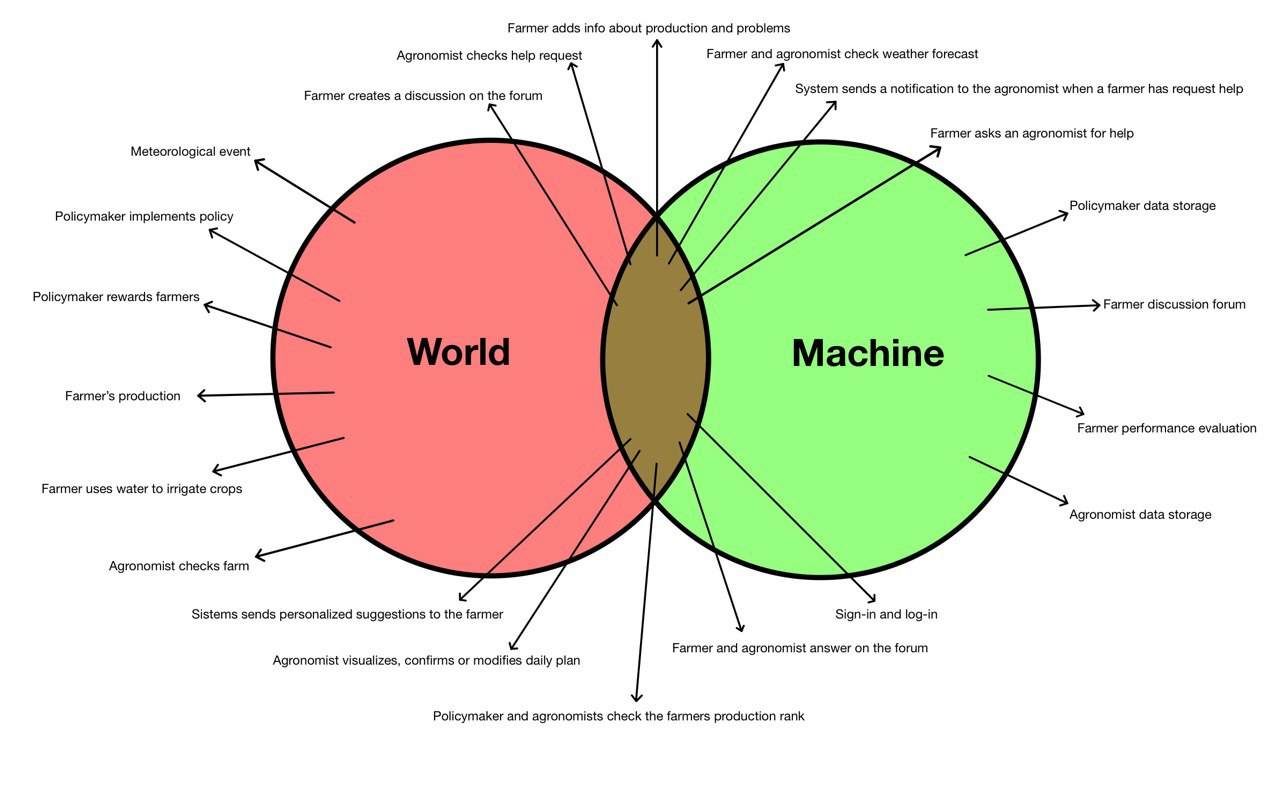
\includegraphics[width=\textwidth,height=\textheight,keepaspectratio]{Images/WorldAndMachine.jpg}
    \caption{The World and the Machine diagram}
    \label{fig:WorldAndMachine}
\end{figure}

\subsubsection{World phenomena}
\begin{itemize}
    \item Meteorological event
    \item Policymaker implements policy
    \item Policymaker rewards farmers
    \item Farmer's production
    \item Farmer uses water to irrigate crops
    \item Agronomist checks farm
\end{itemize}

\subsubsection{Machine phenomena}
\begin{itemize}
    \item Policymaker data storage
    \item Farmer discussion forum
    \item Farmer performance evaluation
    \item Agronomist data storage
\end{itemize}

\subsubsection{Shared phenomena}
\paragraph{Controlled by the World}
\begin{itemize}
    \item Policymaker and agronomist check the farmers production leaderboard
    \item Policymaker sign-in and log-in
    \item Farmer answers help request on the forum
    \item Farmer sign-in and log-in 
    \item Farmer add information about his production
    \item Farmer add information about a problem he faces
    \item Farmer create a discussion on the forum about a problem
    \item Farmer checks weather forecasts
    \item Farmer asks an agronomist for help
    \item Agronomist sign-in and log-in
    \item Agronomist checks help requests
    \item Agronomist answers help request on the forum
    \item Agronomist answers privately help request
    \item Agronomist checks weather forecasts
    \item Agronomist visualizes daily plan
    \item Agronomist confirms or modifies daily plan
\end{itemize}

\paragraph{Controlled by the Machine}
\begin{itemize}
    \item System sends personalized suggestions to the farmer
\end{itemize}

\subsubsection{Goals}

\begin{description}
    \item [G1] Policymakers shall be able to know if steering initiative produced significant results
    \item [G2] Policymakers shall be able to know the best and the worst farmer
    \item [G3] Farmers shall be able to communicate with peers
    \item [G4] Farmers shall be able to send an help request to an agronomist
    \item [G5] Farmers shall received personalized suggestions
    \item [G6] Farmers shall be able to check weather forecasts
    \item [G7] Farmers shall be able to add information about production and problems
    \item [G8] Farmers shall be able to create discussion on the forum
    \item [G9] Agronomists shall be able to visualize, confirm and modify their daily plan
    \item [G10] Agronomists shall be able to help farmers with problems
    \item [G11] Agronomists shall be able to know the best and the worst farmer
\end{description}

\subsection{Definitions, Acronyms, Abbreviations}

\subsubsection{Definitions}

\subsubsection{Acronyms}

\subsubsection{Abbreviations}

\subsection{Revision history}

\subsection{Reference documents}
\begin{description}
    \item [WeBeeP channel] - Project Assignment
    \item [The World \& The Machine] - M. Jackson, P. Zave 
\end{description}

\subsection{Document structure}


%------------------------------------------------------------------------------------------------------------------------------------------------
\clearpage
{\color{Blue}{\section{Overall Description}}}
\label{sect:overview}
\subsection{Product perspective}
\subsubsection{Class diagram}
This section will present the high-level UML class diagrams of the application.
\\\\
\begin{figure}[H]
    \centering
    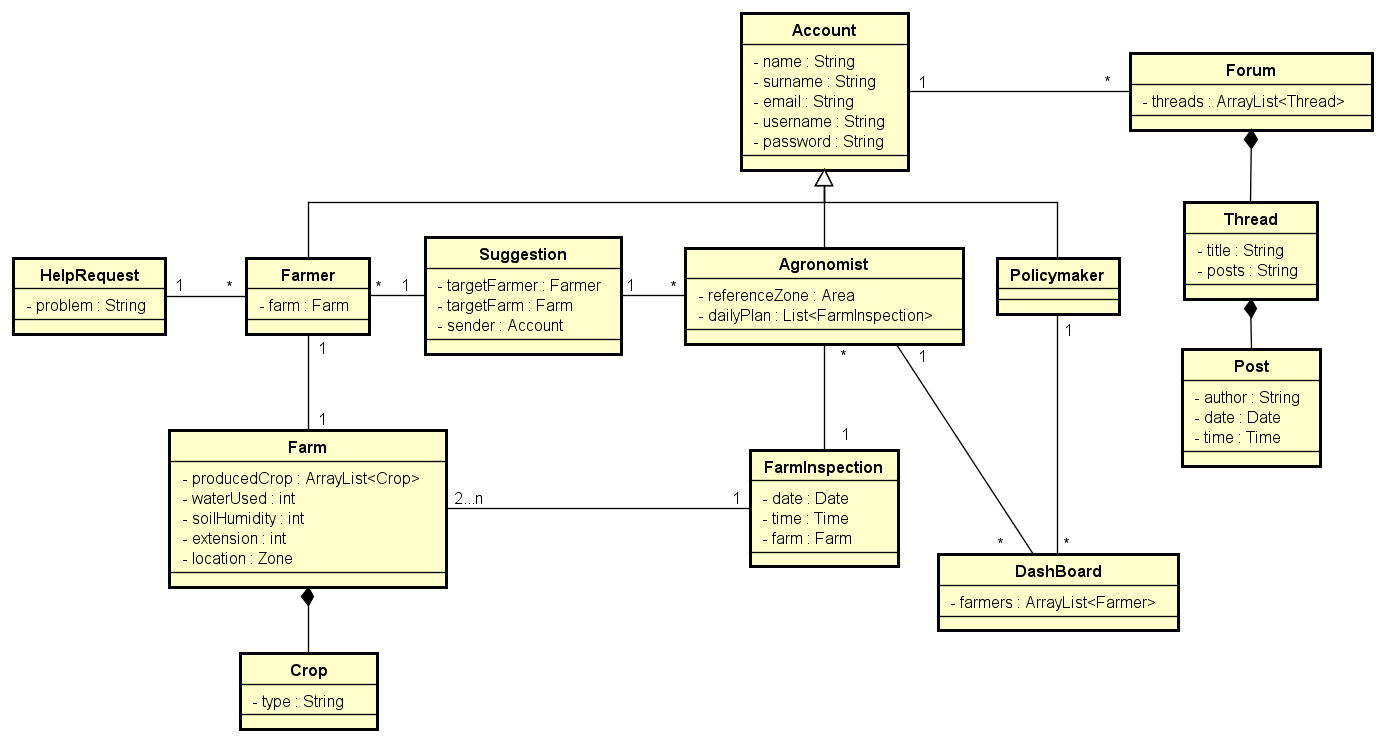
\includegraphics[width=\textwidth,height=\textheight,keepaspectratio]{Images/HighLevelUMLcut.png}
    \caption{\label{fig:high_level_uml}High level class diagram}
\end{figure}

\bigskip
\paragraph{Additional notes on the class diagram}
\begin{itemize}
    \item The agronomist attribute dailyPlan is a collection of FarmInspection ordered by date and time
    \item Agronomists can create a suggestion responding to a farmer help request
\end{itemize}

\newpage
\subsubsection{State machine diagrams}
The following diagrams are meant to give a high-level description of the states' evolution during the system processes.
\\\\

\begin{figure}[H]
    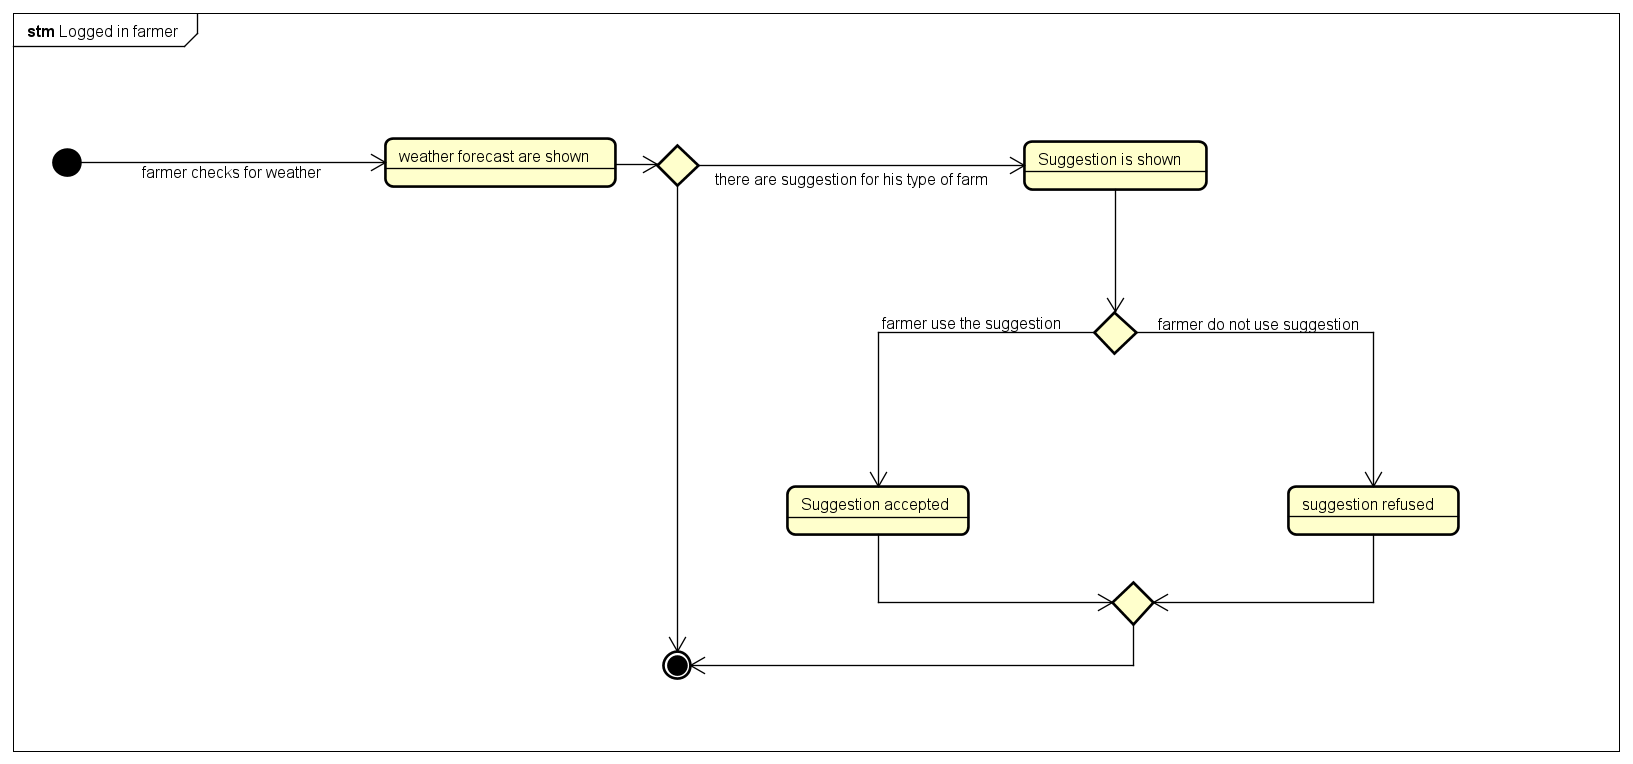
\includegraphics[width=\textwidth,height=\textheight,keepaspectratio]{Images/farmerChecksWeather.png}
    \caption{Statechart of a farmer checking weather forecast}
    \label{fig:statechart_farmer_weather}
\end{figure}

\begin{figure}[H]
    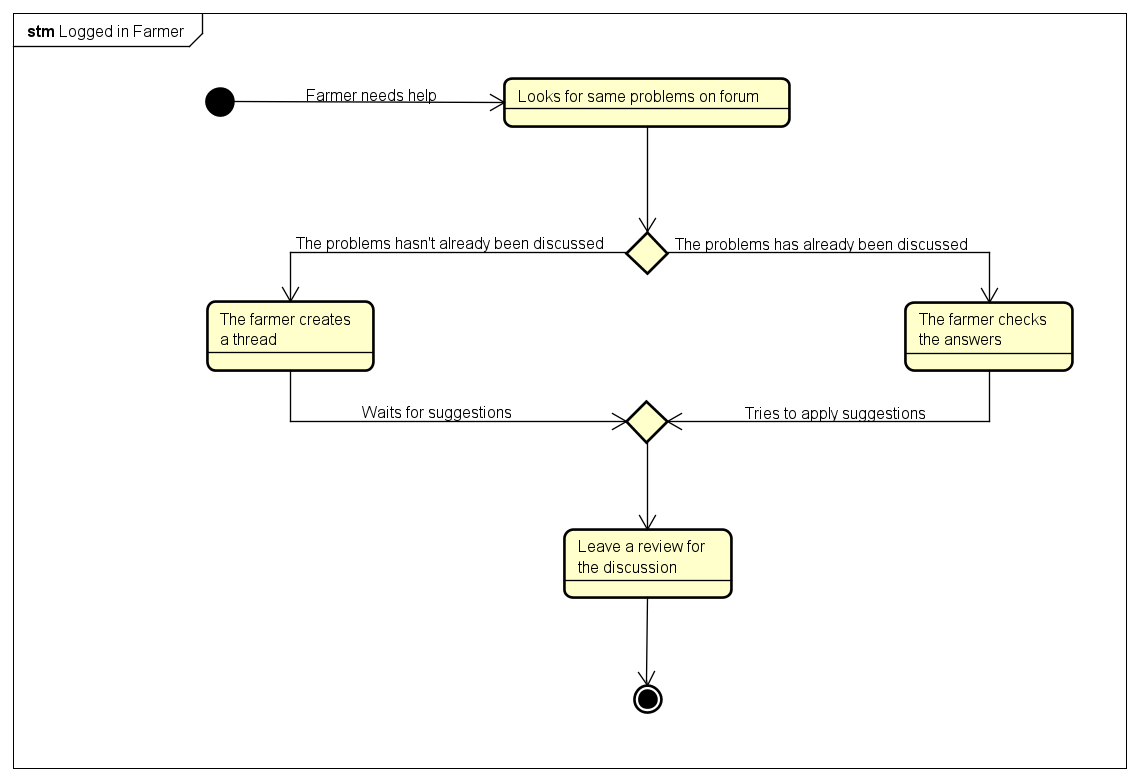
\includegraphics[width=\textwidth,height=\textheight,keepaspectratio]{Images/farmerCreatesThread.png}
    \caption{Statechart of the lifetime of a discussion thread on the forum}
    \label{fig:statechart_farmer_thread}
\end{figure}

\begin{figure}[H]
    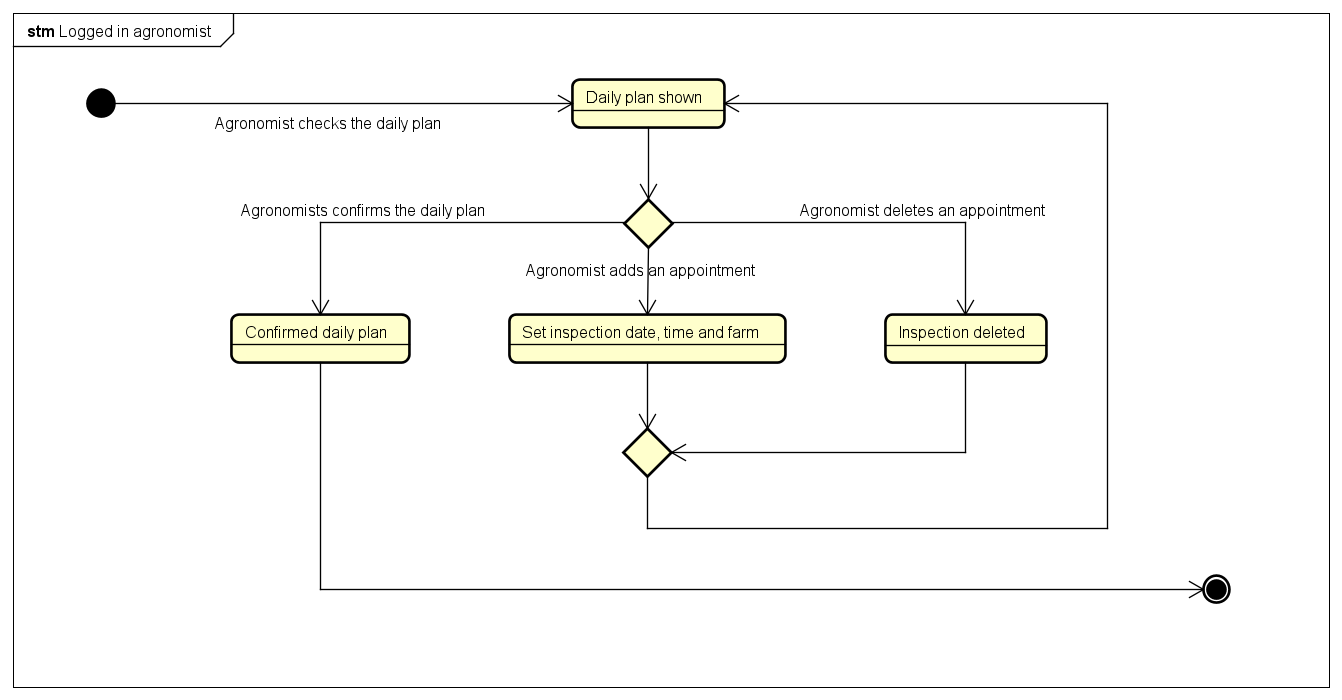
\includegraphics[width=\textwidth,height=\textheight,keepaspectratio]{Images/agronomistDailyPlan.png}
    \caption{Statechart of an agronomist managing his daily plan}
    \label{fig:statechart_agronomist_plan}
\end{figure}

\bigskip
\begin{figure}[H]
    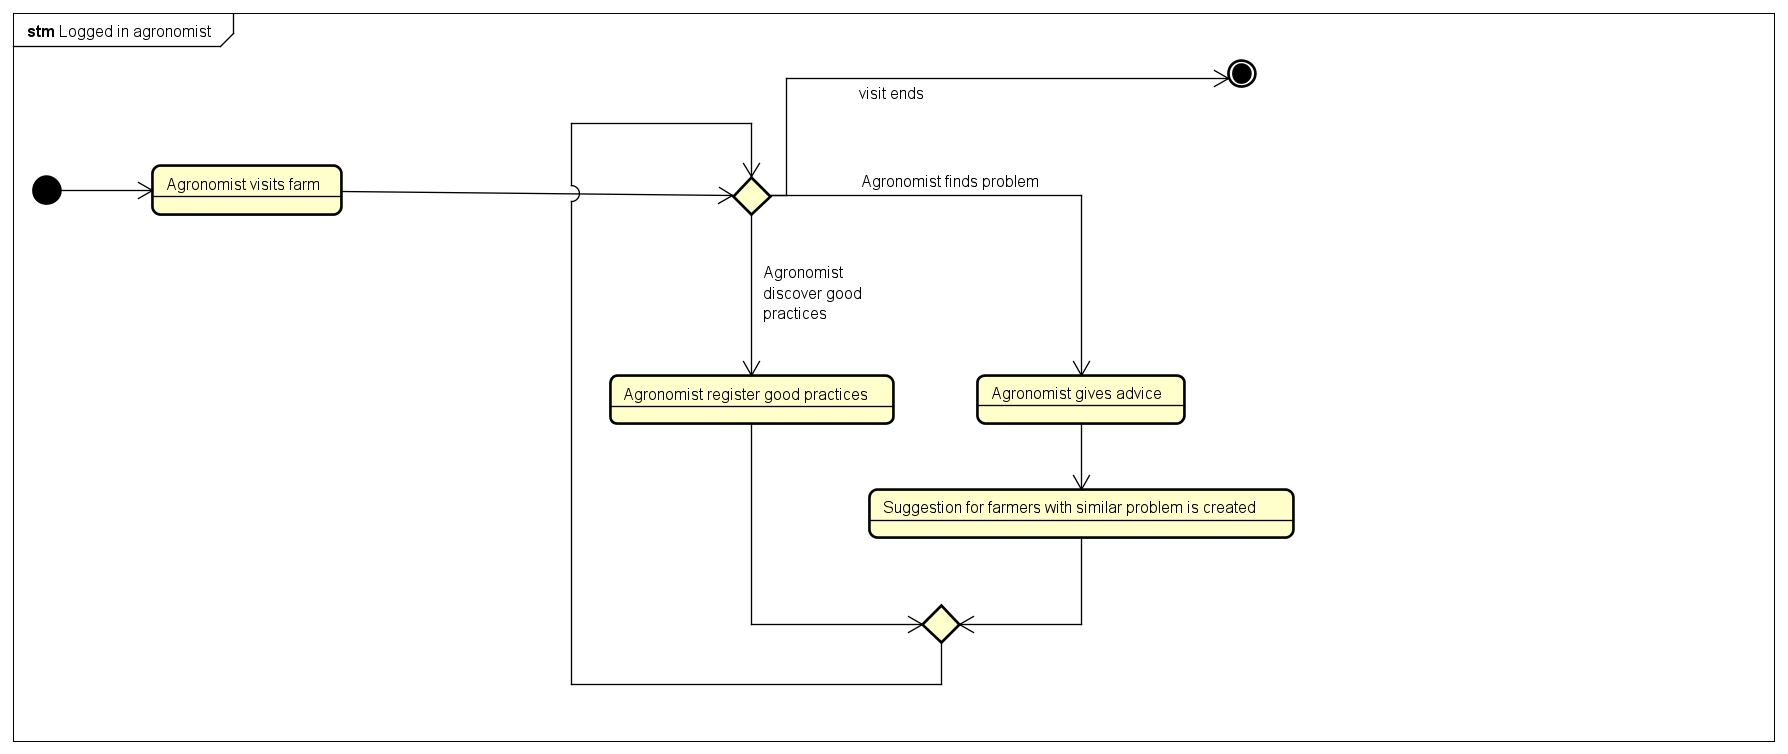
\includegraphics[width=\textwidth,height=\textheight,keepaspectratio]{Images/agronomistVisitFarm.png}
    \caption{Statechart of the lifetime of a farm visit}
    \label{fig:statechart_agronomist_visit}
\end{figure}

\newpage
\subsection{Product functions}
\emph{DREAM} offers Farmers the ability to ask for help from other farmers or an agronomist, 
they can check the weather forecast and see if there are suggestions for them. 
\emph{DREAM} create a leaderboard of the farmers that both agronomist and policymakers can visualize. 
The first ones can discover good practices and help farmers that are performing badly, 
policymakers instead can see the best farmer, reward them and see if the ones who accepted 
suggestions are performing better. 
In addition, \emph{DREAM} offers agronomists the possibility of visualizing, modifying or confirming their daily plan.

\paragraph{Common user functions} These functions are available to all Users:
\begin{itemize}
    \item \textbf{Registration and Login}\\
          User should be able to create a personal account for the App using personal email and password.
          In this process he has to select his role.
          \newline By logging in with their account, user can access the other functions.
\end{itemize}

\paragraph{Basic Farmer functions} These functions are available to all logged-in Farmers:
\begin{itemize}
    \item \textbf{Check weather forecast}\\
          \emph{DREAM} retrieves meteorological short-term and long-term data from an external source and makes them available 
          to farmers. They can check the forecasts on the app and if there are suggestions for their farm these are shown to them.
           These suggestions are created when an agronomist helps a farmer in a similar situation.
    \item \textbf{Request help}\\
          A farmer in case of a problem can ask for the direct help of an agronomist. He can use a section to send a help request,
           when this functionality is used a notification is sent to the agronomist responsible for the location of the farm with informations about the problem and the farm.
    \item \textbf{Create discussion on forum}\\
         \emph{DREAM} has a forum section on which farmers can create a discussion specifying the type of problem and eventual specificity of their farm. 
    \item \textbf{Reply to forum discussion}
        After access to the forum section of \emph{DREAM}, the farmer can select a recent, not closed discussion and post a reply.
    \item \textbf{Close a discussion}
        A farmer after receiving an effective reply can mark the answer as effective and close the discussion.
    \item \textbf{Insert production data}
        A farmer periodically insert in the app the amount of crops produced, the type and the amount of water used.
\end{itemize}

\paragraph{Agronomist base functions}
These functions should be accessible to all logged-in Agronomists
\begin{itemize}
    \item\textbf{Insert area he is responsible for}\\
    From the home page, the agronomist can open a geographical representation of Telangana
    and select the area he is responsible for. \emph{DREAM} checks if the selected territory is already overseen
    by another agronomist. In that case, the app asks the user to repeat the process;
    otherwise, the selection is saved on \emph{DREAM}'s database.
    \item \textbf{Reply to forum discussion}\\
    After access to the forum section of \emph{DREAM}, the agronomist can select a recent,
    not closed discussion and post a reply.
    \item \textbf{Reply to help request}\\
    On receiving a private help request from a farmer, the agronomist receives a
    notification containing the sender and the problems they need to face.
    \item \textbf{Visualize information area}\\
    \emph{DREAM} retrieves meteorological short-term and long-term data from an external source
    and makes them available to agronomists on the app.
    \newline In addition, \emph{DREAM} offers the possibility to the agronomist of visualizing the best
    performing farmers in his related area; these farmers are selected through thresholds
    (concerning the production and especially the resilience to meteorological adverse events)
    created by the agronomist of the corresponding area.
    \item\textbf{Daily plan management}\\
    From his personal area, the agronomist can visualize the daily plan on a calendar.
    The user has three possible choices: add or delete an appointment and confirm the plan;
    the first two can be repeated several times until the confirmation. In case of deletion of a visit with a given farmer,
    \emph{DREAM} reinserts automatically the same appointment, according to the agronomist's availability,
    only if with that farmer there are less than two visits planned for this year.
    \newline The app suggests to the agronomists the farmers that are under-performing thus need to be visited more often.
    \newline At the end of each day, the agronomist has to confirm the execution of the daily plan or specify
    the deviations from that.
    \item\textbf{Insert good practices}\\
    The agronomist after the visit to a farm can add good practices
    that will be available to farmers with similar conditions and crops.
\end{itemize}

\paragraph{Basic Policy maker functions} These functions are available to all logged-in Policy makers:
\begin{itemize}
    \item \textbf{Visualize farmers' performance}\\
    DREAM provides policy makers with a dashboard with comprehensive data about farmers in Telangana.
    The dashboard shows for each area the farmers that are performing well, the ones who are performing badly,
    and the ones who are exceeding the thresholds by far (the last ones are those who will receive special incentives).
    \newline In addition, there is a section that shows the result of farmers who recently received help.
\end{itemize}

\newpage
\subsection{User characteristics}

DREAM is meant to be accessible for both specialized and unspecialized users.

\paragraph{Users}
\begin{itemize}
    \item \textbf{Farmer}: people that own a farm and may need help
    \item \textbf{Agronomist}: someone who is specialized in agriculture activity and is responsible for a given area
    \item \textbf{Policy maker}: people who oversight the agriculture process of Telangana
\end{itemize}

\bigskip
\subsection{Assumptions, dependencies and constraints}
\begin{description}
    \item[D1] Each user creates only one account
    \item[D2] The information provided by the farmer is correct
    \item[D3] The thresholds provided by the agronomists are reasonable for the zone they are responsible for
    \item[D4] Most of the farmers that receive suggestions will enact them
    \item[D5] The answers to the forum's threads are consistent
    \item[D6] A privately help request to an agronomist is replied
    \item[D7] Users will be instructed to use the application if possible
    \item[D8] Agronomist is entitled to choose only his area of responsibility
    \item[D9] Each area has only one responsible agronomist 
\end{description}

%------------------------------------------------------------------------------------------------------------------------------------------------
\clearpage
{\color{Blue}{\section{Specific Requirements}}}
\label{sect:requirements}
\subsection{External interface Requirements}
The \emph{DREAM} frontend is a web application that can be accessed from web browsers, both from mobile and
desktop devices. The following section will give a comprehensive description in terms of hardware, software
and communication interfaces.

\bigskip
\subsubsection{Common users interfaces}
\textbf{Login and Registration}\\
When first opening the application, all the users are presented with the login page. If not already registered,
it is provided a registration button. In this section they are asked to provide: first name, second name,
a \emph{username}, an \emph{e-mail address} and a \emph{password}. The interface also shows a small button to switch
to the login page, in case the user has already signed in on another device or the session has expired.

\bigskip
\begin{figure}[H]
    \centering
    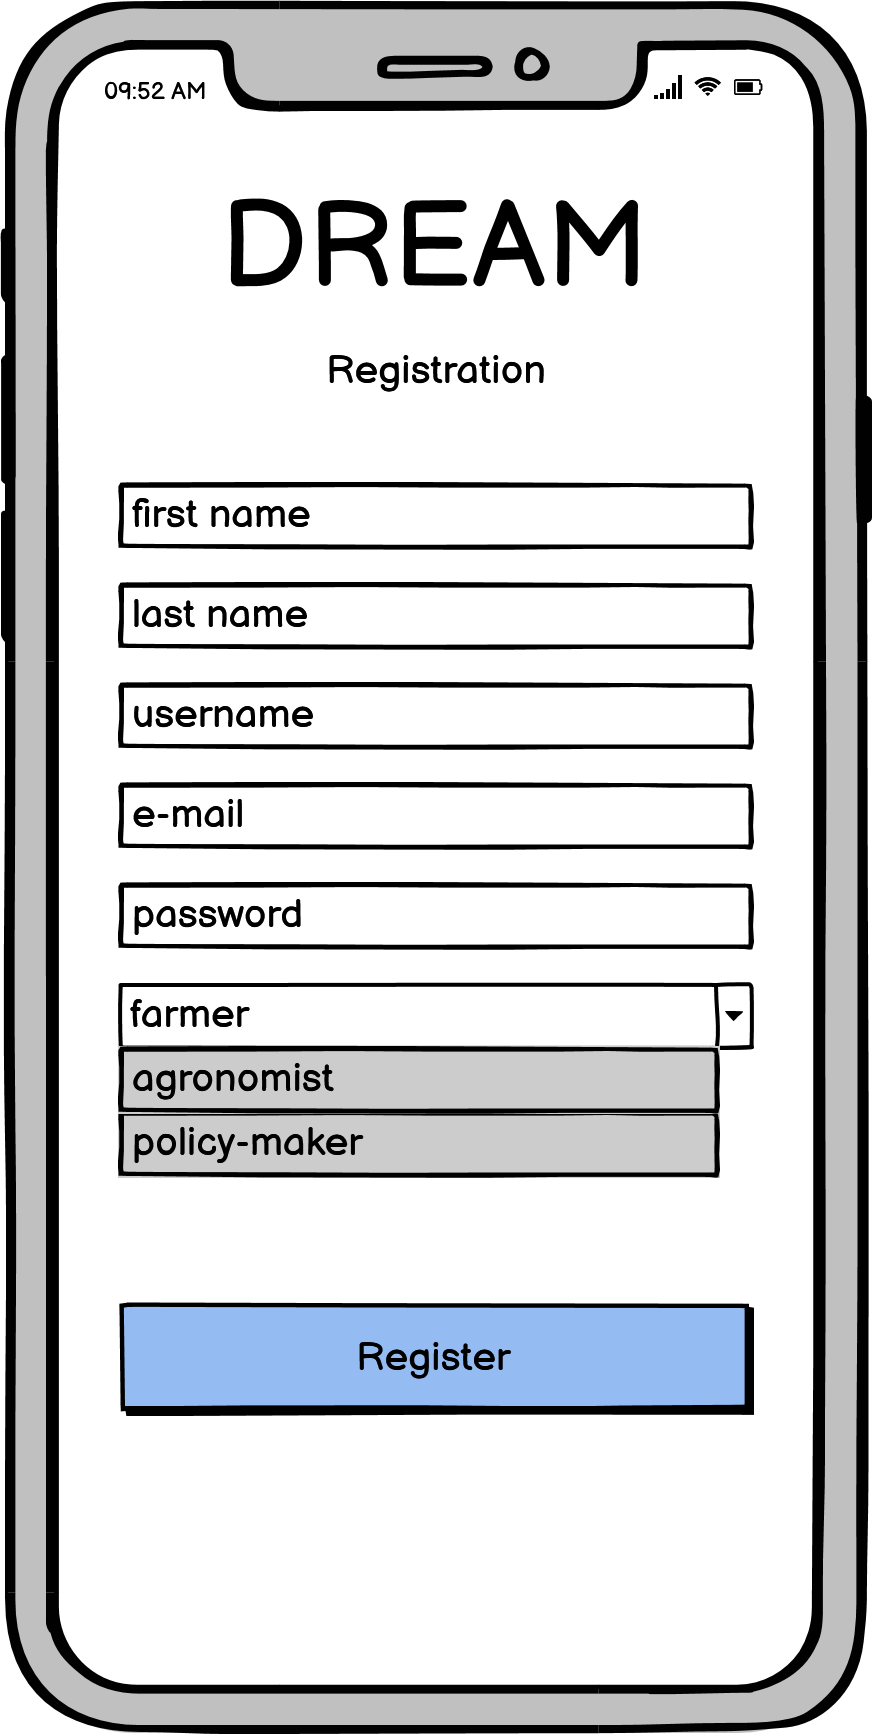
\includegraphics[scale=0.40]{Images/registration.png}
    \caption{Registration interface}
\end{figure}

\newpage
\begin{figure}[H]
    \centering
    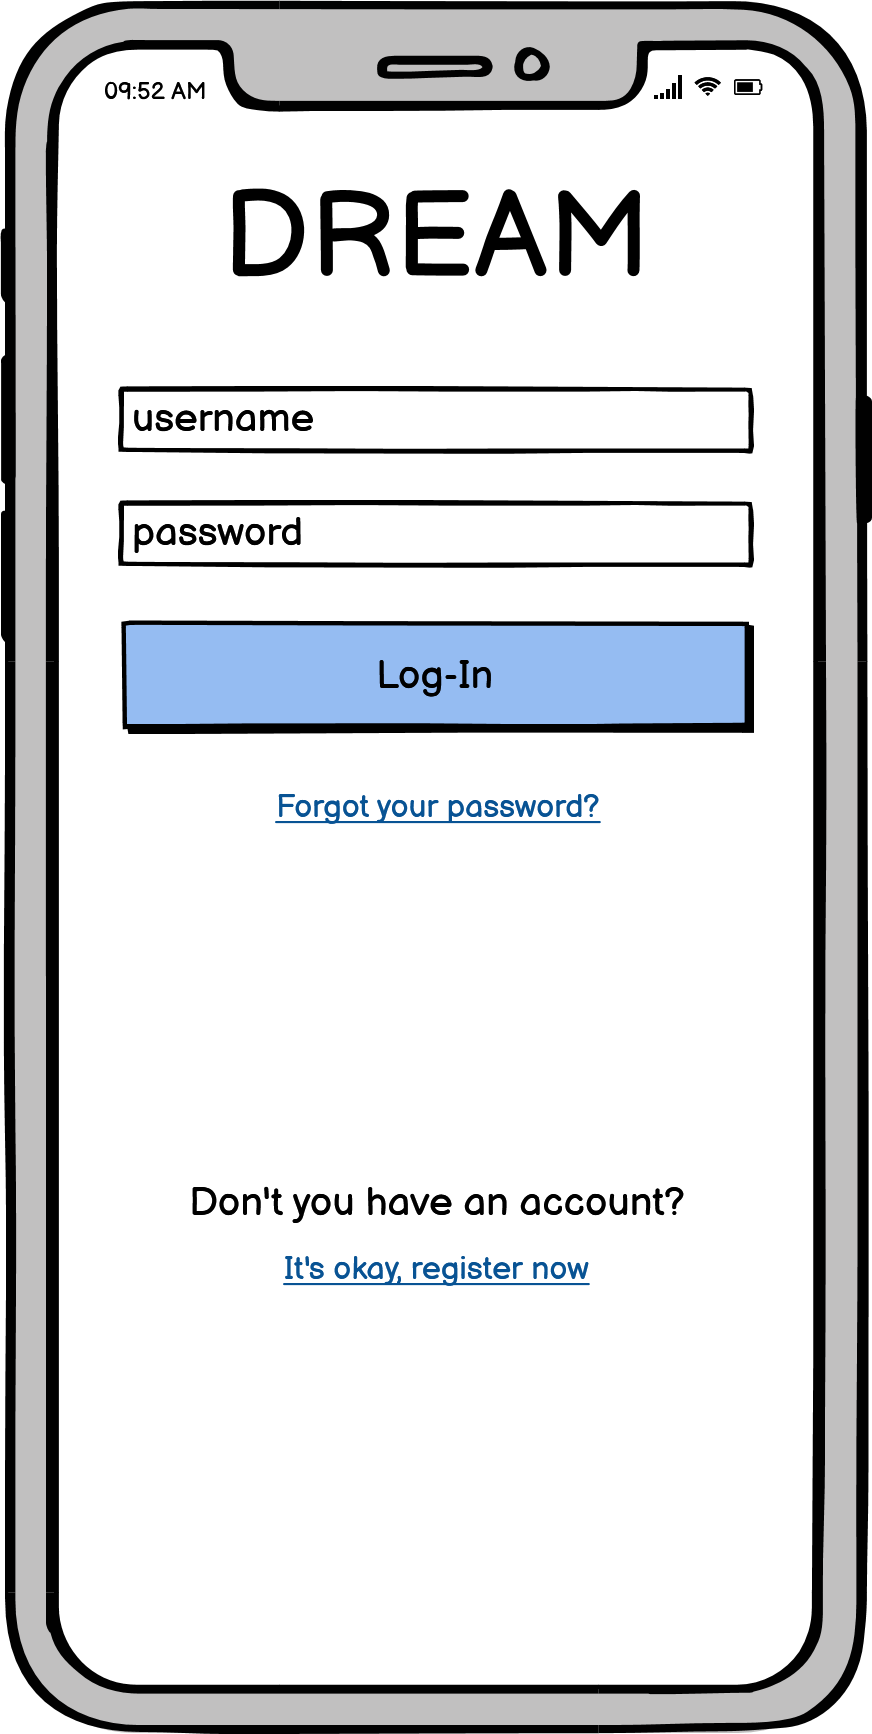
\includegraphics[scale=0.40]{Images/log-in.png}
    \caption{Log-in interface}
\end{figure}

\textbf{Farmer's home page} \\
Provides different options. The user can insert data concerning production,
checks weather forecasts, privately request help, and reach the forum.
\begin{figure}[H]
    \centering
    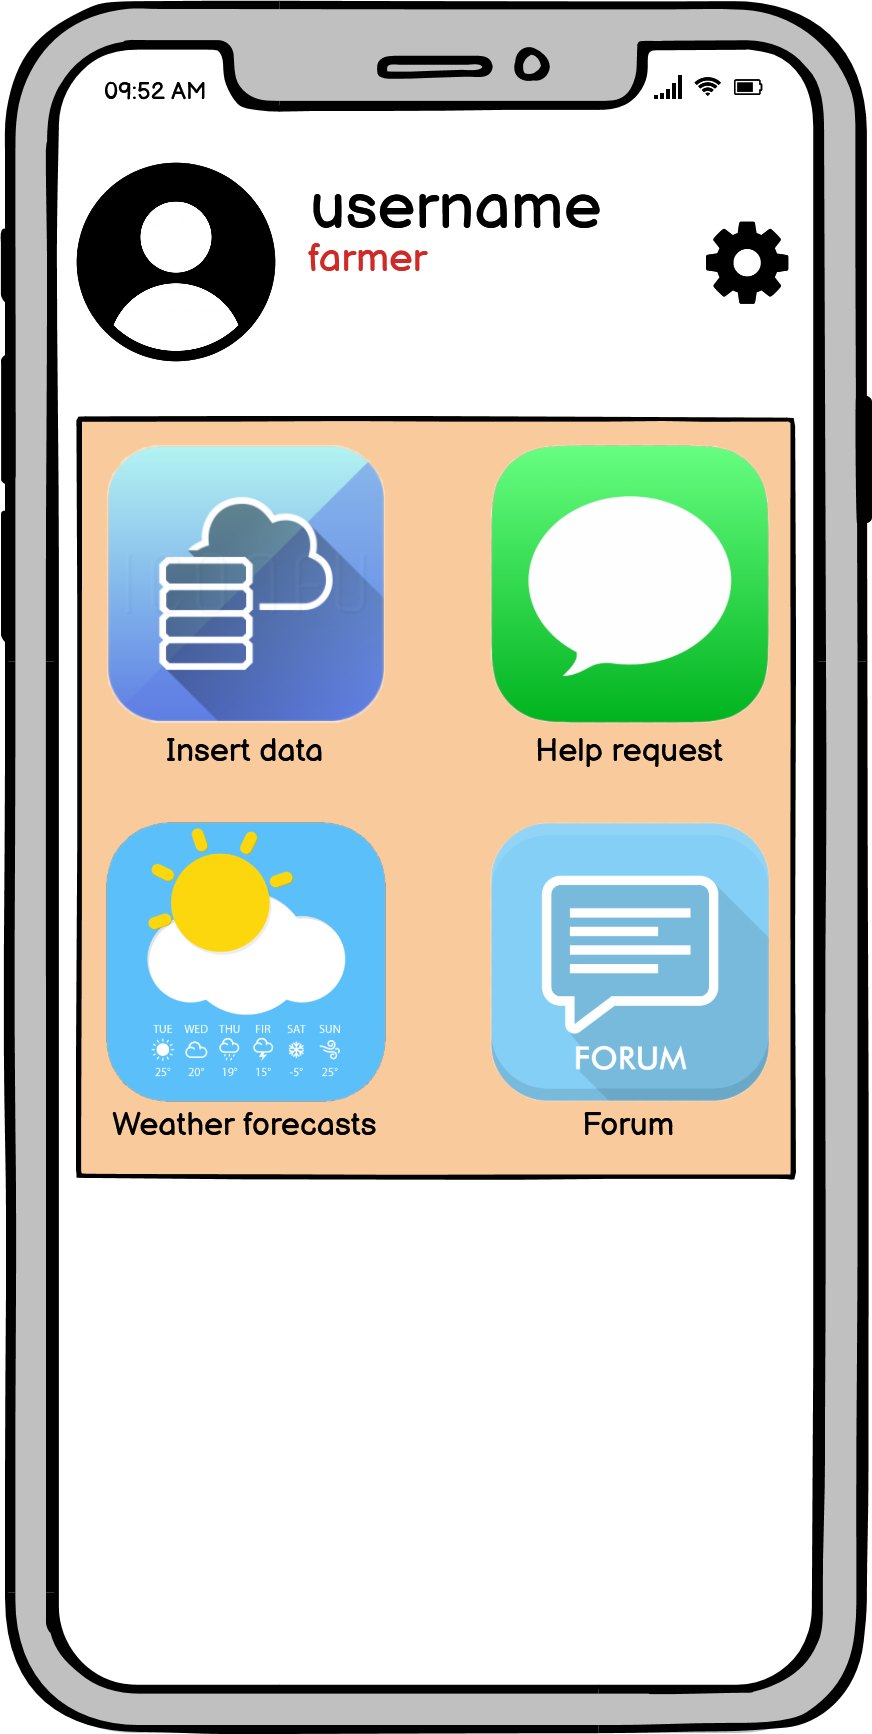
\includegraphics[scale=0.45]{Images/farmerHomePage.png}
    \caption{Farmer's home page}
\end{figure}

\textbf{Agronomist's home page} \\
Provides the possibility of selecting the area of responsibility, answering private help requests,
checking the weather, accessing the forum, managing the daily plan, and checking the dashboard
\begin{figure}[H]
    \centering
    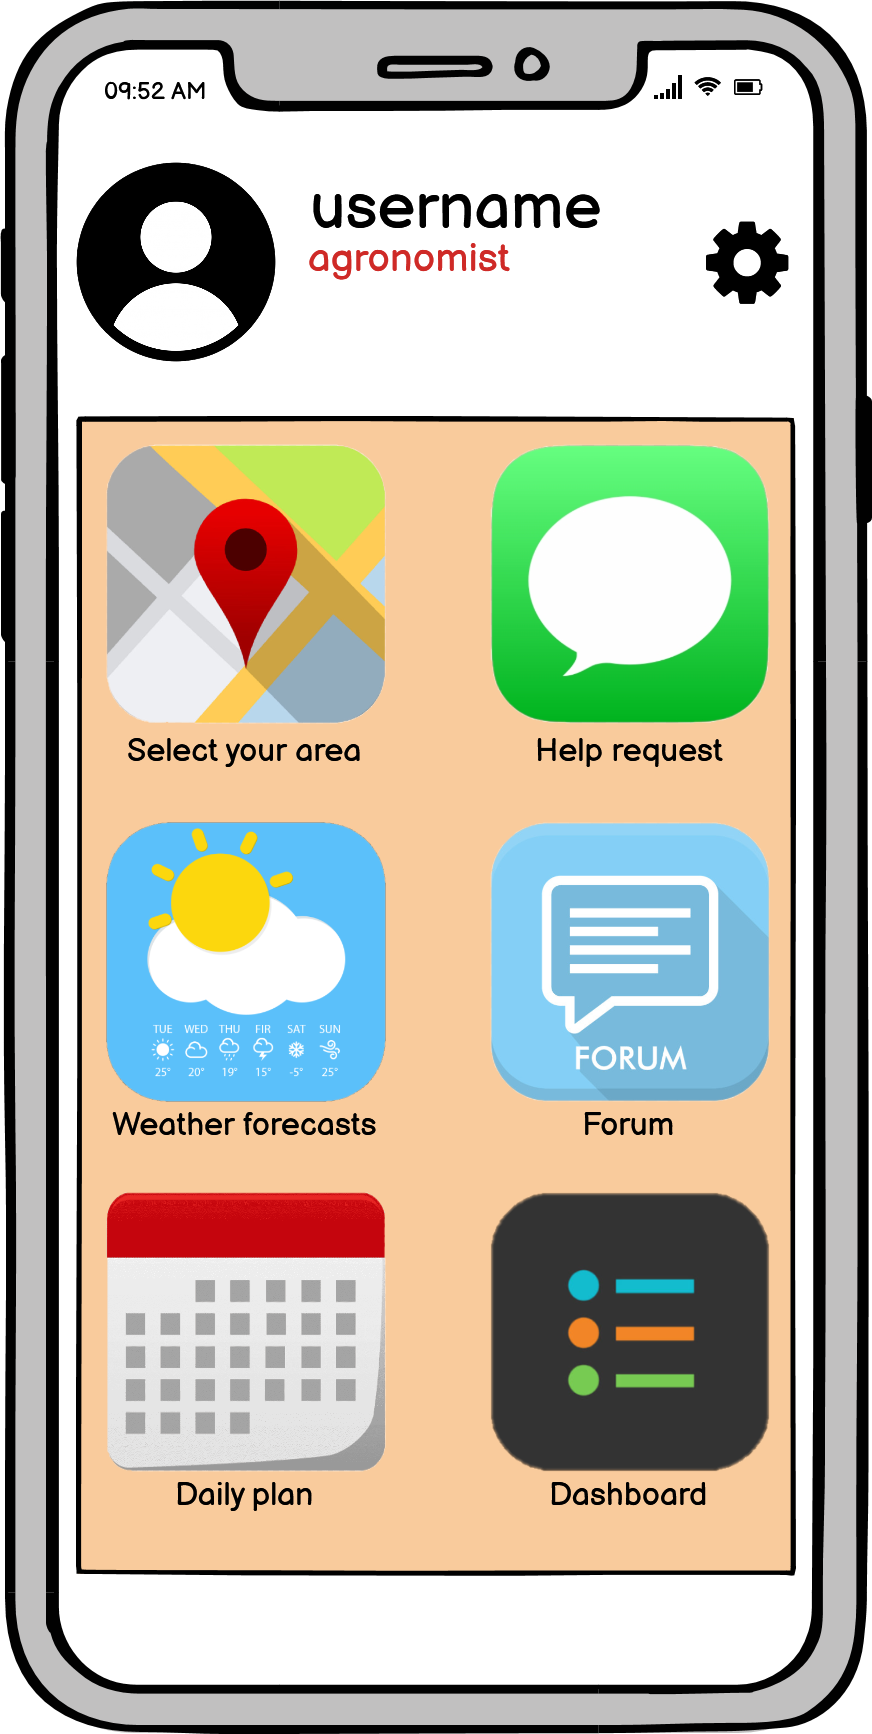
\includegraphics[scale=0.40]{Images/agronomistHomePage.png}
    \caption{Agronomist's home page}
\end{figure}

\textbf{Policymaker's home page} \\
Provides a table containing values for all farmers in the system. Every field of this table can be ordered.
\newline There are also graphs that sum up data about production.
\begin{figure}[H]
    \centering
    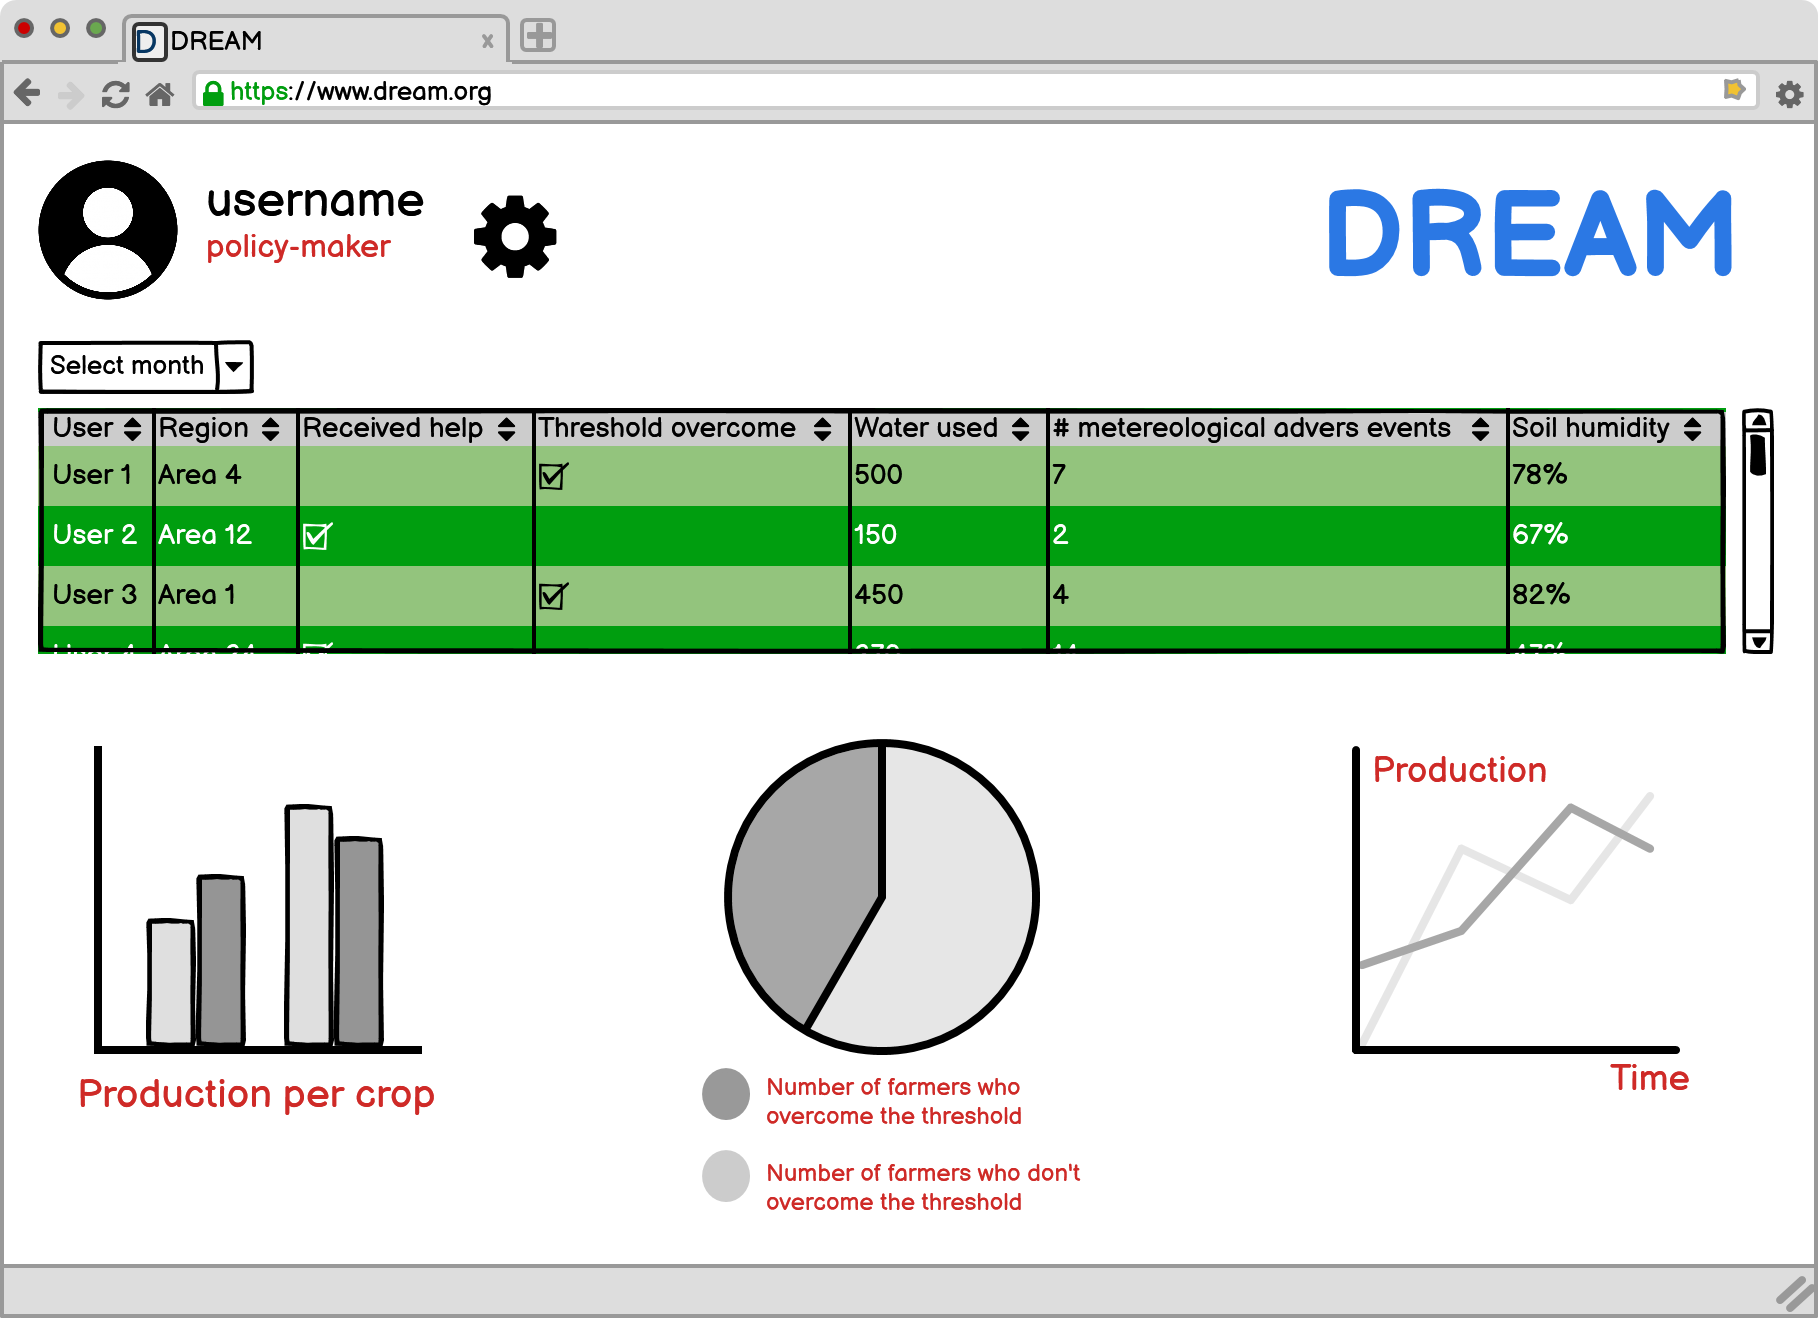
\includegraphics[scale=0.40]{Images/policymakerHomePage.png}
    \caption{Policymaker's home page}
\end{figure}

\newpage
\textbf{Forum - home page} \\
The forum section is accessible to both the farmers and the agronomists. Agronomists have the possibility
of taking a look at the requests and answer to them. Farmers, as agronomists, can answer to the forum threads
but can also create a new discussion.
\begin{figure}[H]
    \centering
    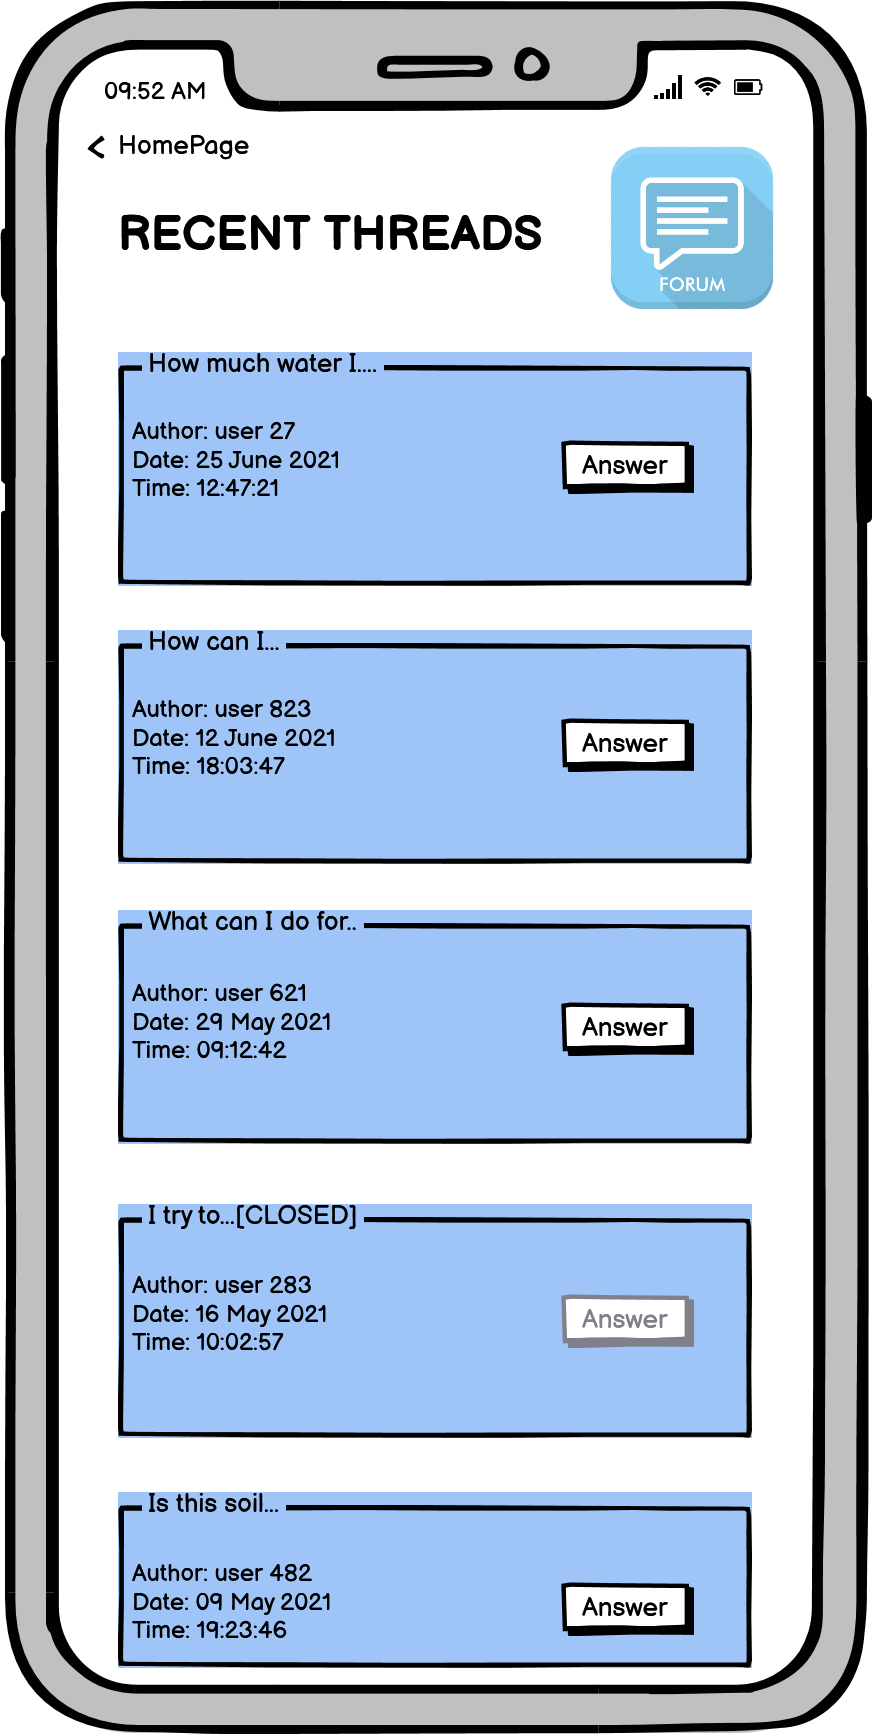
\includegraphics[scale=0.40]{Images/agronomistForum.png}
    \caption{Agronomist's forum home page}
\end{figure}
\bigskip
\begin{figure}[H]
    \centering
    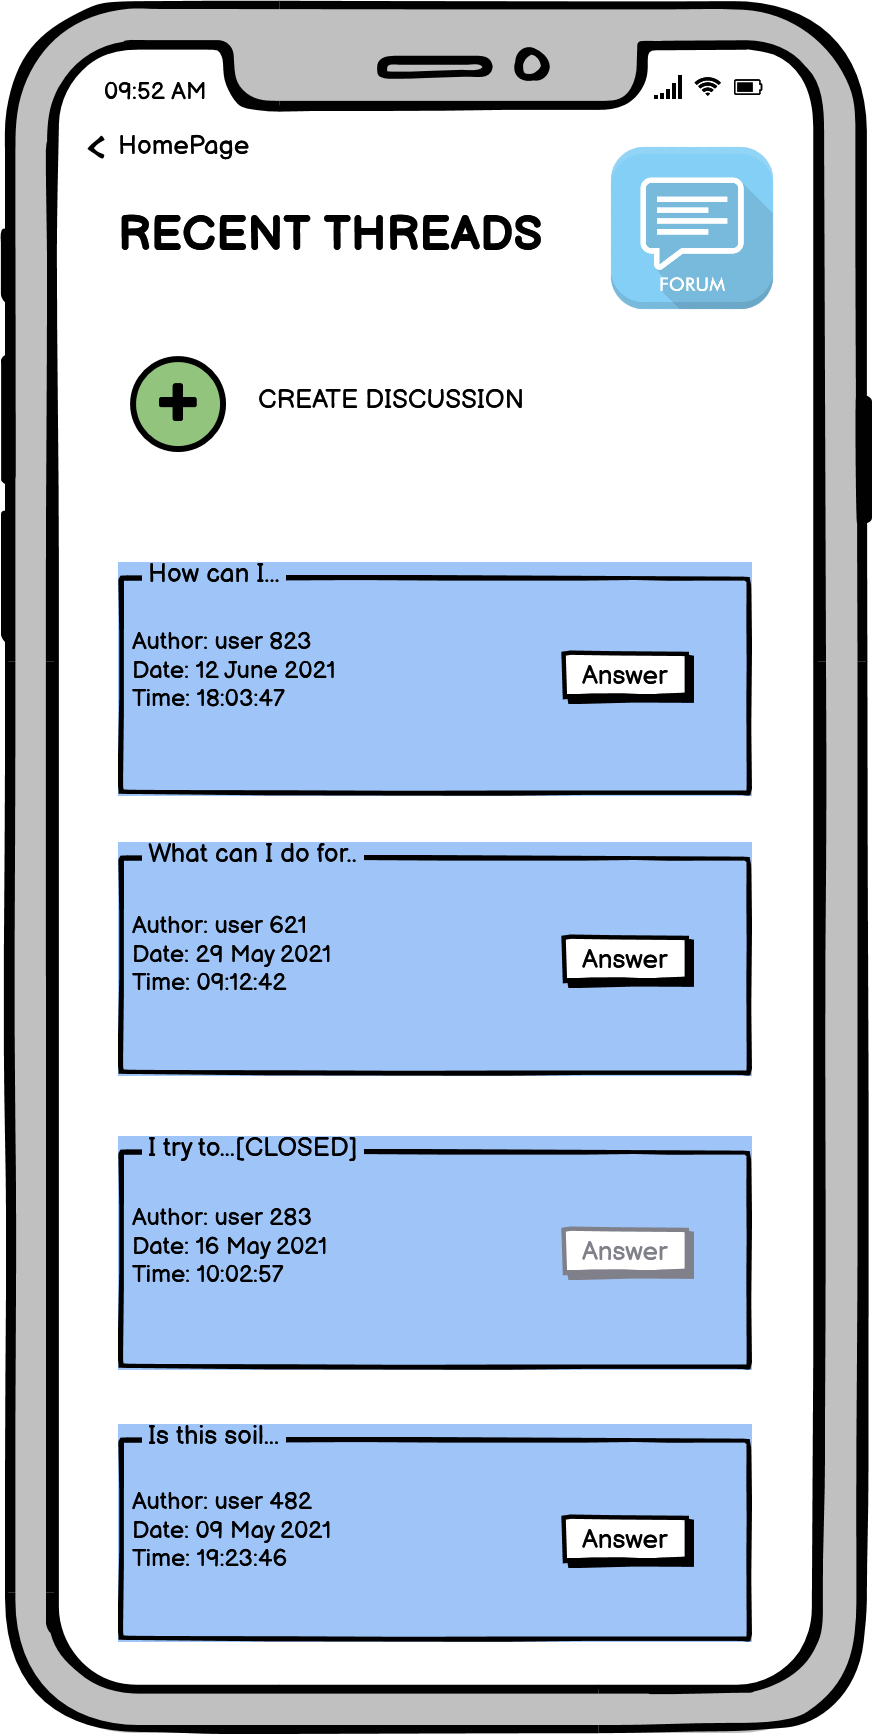
\includegraphics[scale=0.40]{Images/farmerForum.png}
    \caption{Farmer's forum home page}
\end{figure}

\newpage
\textbf{Daily plan - home page} \\
The daily plan home page presents a calendar in which appointments day are marked in red.
By clicking on a date is possible to manage it, by adding or removing an appointment.
\begin{figure}[H]
    \centering
    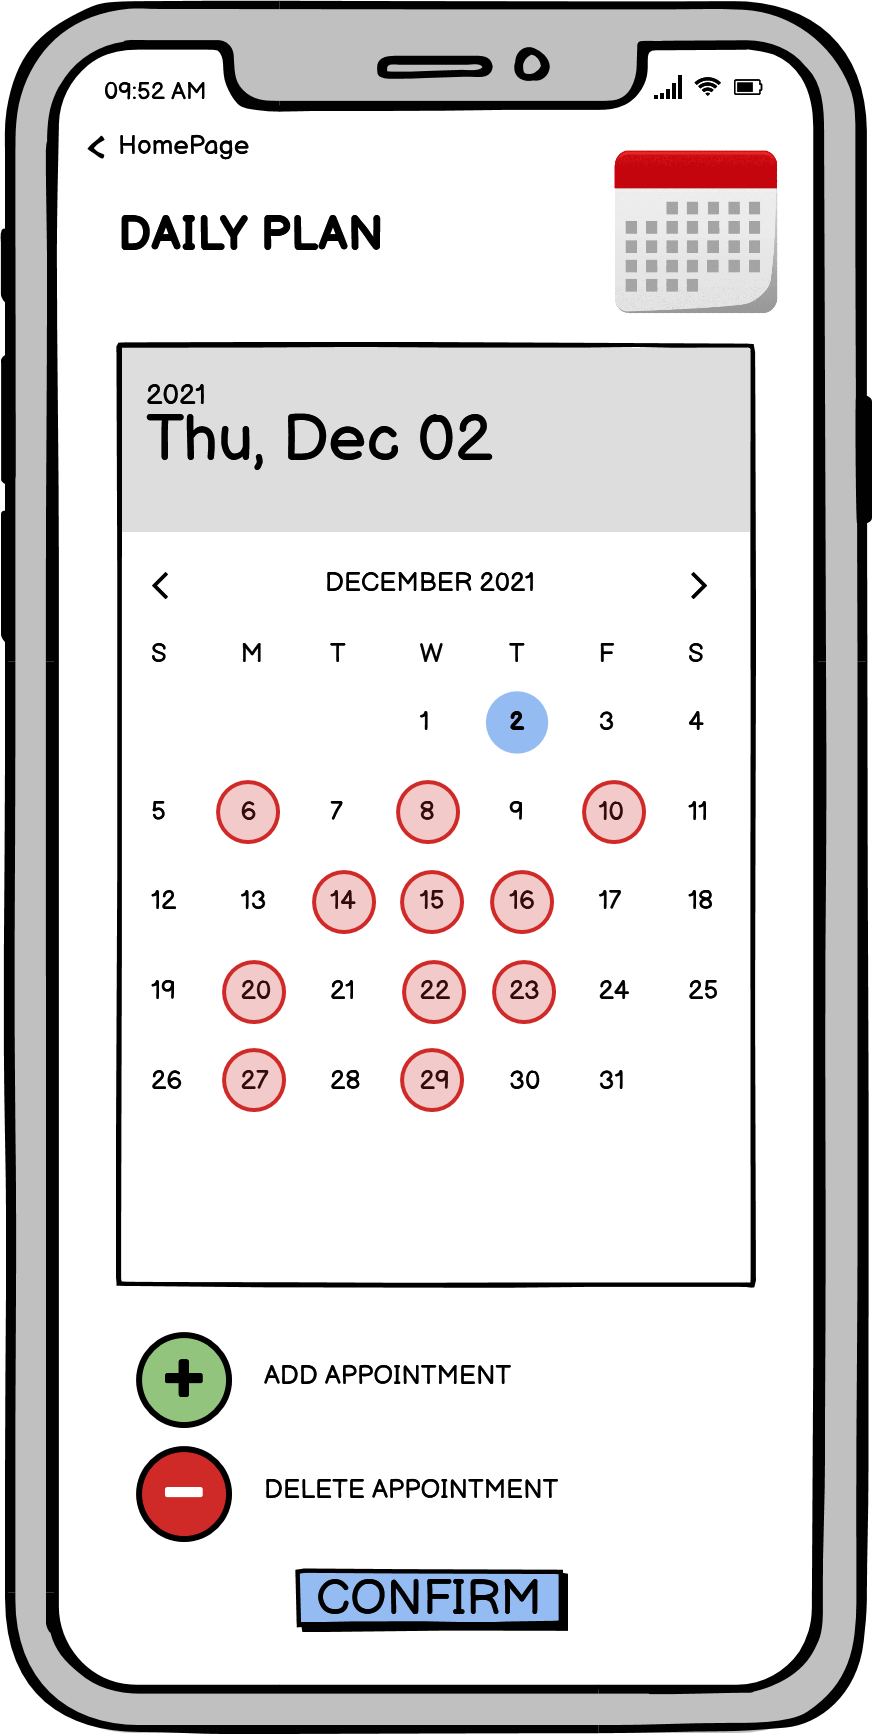
\includegraphics[scale=0.40]{Images/dailyplan.png}
    \caption{Daily plan management home page}
\end{figure}


\bigskip
\subsection{Functional Requirements}
\subsubsection{Goal-Requirement mapping}
\begin{description}
    \item [G1] Policymakers shall be able to know if steering initiative produced significant results
        \begin{description}
            \item[R1] The system shall keep track of the farmer who requested help and of the suggestion that they received
            \item[R2] The system shall keep track of historical data for each zone
            \item[R3] The system shall keep track of meteorological events
            \item[R4] Farmers shall be able to create a help request specifying  the type of problem
            \item[R5] The system shall be able to record data about production inserted by the farmer
            \item[R6] Agronomist shall be able to insert significant prodution thresholds for each zone   
        \end{description}
    \item [G2] Policymakers shall be able to know the best and the worst farmer
        \begin{description}
            \item[R2] The system shall keep track of historical data for each zone
            \item[R3] The system shall keep track of meteorological events
            \item[R5] The system shall be able to record data about production inserted by the farmer
            \item[R6] Agronomist shall be able to insert significant prodution thresholds for each zone   
        \end{description}
    \item [G3] Farmers shall be able to communicate with peers
        \begin{description}
            \item[R7] Farmers shall be able to create discussion threads on the forum
            \item[R8] Farmers shall be able to reply to discussion on the forum
            \item[R13] The system shall be able to manage a forum
        \end{description}
    \item [G4] Farmers shall be able to send an help request to an agronomist
        \begin{description}
            \item[R1] The system shall keep track of the farmer who requested help and of the suggestion that they received
            \item[R4] Farmers shall be able to create a help request specifying  the type of problem
            \item[R9] The system shall send a notification to the Agronomists when a farmer has requested help
        \end{description}
    \item [G5] Farmers shall received personalized suggestions
        \begin{description}
            \item[R1] The system shall keep track of the farmer who requested help and of the suggestion that they received
            \item[R2] The system shall keep track of historical data for each zone
            \item[R3] The system shall keep track of meteorological events
            \item[R5] The system shall be able to record data about production inserted by the farmer
            \item[R6] Agronomists shall be able to insert significant prodution thresholds for each zone
            \item[R10] After an agronomist has registered a best practice or a suggestion to a farmer, the system should infer the farmers with similar characteristics and send them the same suggestion 
        \end{description}
    \item [G6] Farmers shall be able to check weather forecasts
        \begin{description}
            \item[R3] The system shall keep track of meteorological events
            \item[R11] The systems shall be able to connect to an external service to retrieve meteorological forecasts
            \item[R12] The system shall give Farmer the possibility to see weather forecasts
        \end{description}
    \item [G7] Farmers shall be able to add information about production and problems
        \begin{description}
            \item[R4] Farmers shall be able to create a help request specifying  the type of problem
            \item[R5] The system shall be able to record data about production inserted by the farmer
        \end{description}
    \item [G8] Farmers shall be able to create discussion on the forum
        \begin{description}
            \item[R5] The system shall be able to record data about production inserted by the farmer
            \item[R13] The system shall be able to manage a forum
        \end{description}
    \item [G9] Agronomists shall be able to visualize, confirm and modify their daily plan
        \begin{description}
            \item[R14] The system shall be able to record data about visits of agronomists
            \item[R15] The system shall be able to manage a calendar
            \item[R16] The system shall organize Agronomists' calendar in such a way that they visit each farm at least twice a year
        \end{description}
    \item [G10] Agronomists shall be able to help farmers with problems
    \begin{description}
        \item[R4] Farmers shall be able to create a help request specifying  the type of problem
        \item[R9] The system shall send a notification to the Agronomists when a farmer has requested help
        \item[R10] After an agronomist has registered a best practice or a suggestion to a farmer, the system should infer the farmers with similar characteristics and send them the same suggestion 
    \end{description}
    \item [G11] Agronomists shall be able to know the best and the worst farmer
    \begin{description}
        \item[R2] The system shall keep track of historical data for each zone
        \item[R3] The system shall keep track of meteorological events
        \item[R5] The system shall be able to record data about production inserted by the farmer
        \item[R6] Agronomist shall be able to insert significant prodution thresholds for each zone   
    \end{description}
\end{description}

\bigskip
\subsubsection{Scenarios}
\paragraph{Scenario 1} Daily plan confirmation\\
Tom is an agronomist that has just finished his work shift, so he logs in to the app and clicks on the daily plan icon.
The daily appointment with farmers just completed, follows exactly the plan previously determined, so he presses the
confirmation button.

\bigskip
\paragraph{Scenario 2} Daily plan modification\\
Martha is an agronomist that is planning his appointments with farmers. She logs in to DREAM and, from the home page,
opens the daily plan section; here she decided to remove an appointment planned for the 10th of December selecting the
corresponding date and then the deletion icon that updates the daily plan. After that, Martha, from the calendar,
selects the 28th of December, and then she presses on the addition icon below: doing that another section is opened in
which she can insert information about the appointment to plan (date, time, and the farm that she wants to visit).
Confirming the operation, she will come back to the daily plan section and the daily plan is updated.

\bigskip
\paragraph{Scenario 3} Agronomist's area selection\\
Marvin is an agronomist that has just completed the registration. After the registration and the log in,
he decides to select his area of responsibility from the map icon on the home page. In this area, a political map of
Telangana is shown and Marvin selects his responsibility zone. No errors occur so Marvin can select the confirmation
button and his area is stored.

\bigskip
\paragraph{Scenario 4} Forum discussion creation\\
Anthony is a farmer and has problems with soil humidity in his fields, so he decides to post a question on the forum.
In order to do that, he logs in and clicks on the forum icon. In the forum section, he selects the add discussion icon:
another section is opened in which he writes his question and post it.

\bigskip
\paragraph{Scenario 5} Farmer insert data\\
Jack is a farmer who recently finished collecting his harvest. He opens the app, logs in to the system. On his home page, 
he selects the Insert Data icon, he now can insert the amount and the type of crop he has harvested and then confirm.

\bigskip
\paragraph{Scenario 6} Farmer Help Request\\
Marty is a farmer who is having some problems in the cultivation of a crop and because he can't wait for a response on the 
forum decides to request help from an agronomist. He logs in on the app, selects the request help icon, inserts a brief description 
of the problem and then confirms that he wants to ask for the help of an agronomist. Victor is one of the agronomists responsible 
for the zone of Marty. After Marty's request, he receives a message containing a description of the problem. Victor conveys that the 
problem of Marty is a serious one so he decides to schedule a visit to his farm through the app functionality.

\bigskip
\paragraph{Scenario 7} Policymaker checks performance of farmer who received help\\
Tom is an official of the Telangana Department of Agriculture, after the recent flood he wants to know how many farmers have requested 
help and if this help has been effective. He logs in on the website of DREAM and can see the dashboard with some aggregate data. 
To see which farmers requested help he can select the previous month from the choice box and check which user had requested help, 
then he can see if in the current month the users who received help have overcome the thresholds set by the agronomist. He then wants 
to know who are the best performing farmers so he orders the table to show the users who have the greatest number of meteorological 
events but overcome the threshold nevertheless.

\subsubsection{Use cases}

\begin{table}[H]
    \begin{tabu} to \textwidth {|X|X[4]|}
        \hline
        Name            & User creates an account \\ \hline
        Actor           & User                    \\ \hline
        Entry condition & \begin{itemize}
            \item The User has not created an account yet
            \item The User has to be a farmer, an agronomist or a policy maker
        \end{itemize}  \\ \hline
        Event flow      & \begin{enumerate}
            \item The User opens the app
            \item The app asks for login or registration
            \item The User clicks on \emph{"Register now"}
            \item The User inserts his first name, last name, username, e-mail, password and role
            \item The User clicks on \emph{"Register"}
            \item The app notifies to User that the registration is confirmed
        \end{enumerate}  \\ \hline
        Exit condition  & \begin{itemize}
            \item User account is added to the database
            \item The User can login
        \end{itemize}  \\ \hline
        Exceptions      & \begin{itemize}
            \item The User already exists
        \end{itemize}  \\ \hline
    \end{tabu}
\end{table}

\begin{table}[H]
    \begin{tabu} to \textwidth {|X|X[4]|}
        \hline
        Name            & User logs in           \\ \hline
        Actor           & Registered User        \\ \hline
        Entry condition & \begin{itemize}
            \item The User has an account
        \end{itemize} \\ \hline
        Event flow      & \begin{enumerate}
            \item The User opens the app
            \item The app asks for login or registration
            \item The User inserts their username and password
            \item The User clicks on \emph{"Log-In"}
            \item The User receives confirmation from the server
            \item The Customer is brought to the home page
        \end{enumerate} \\ \hline
        Exit condition  & \begin{itemize}
            \item The User is logged in
            \item The User can use other features
        \end{itemize} \\ \hline
        Exceptions      & \begin{itemize}
            \item The User insert wrong credentials
            \item The insert username doesn't exist in the app database
        \end{itemize} \\ \hline
    \end{tabu}
\end{table}

\begin{table}[H]
    \begin{tabu} to \textwidth {|X|X[4]|}
        \hline
        Name            & User checks weather forecasts and suggestions           \\ \hline
        Actor           & Agronomist and farmer logged-in    \\ \hline
        Entry condition & \begin{itemize}
            \item The User has logged in
        \end{itemize} \\ \hline
        Event flow      & \begin{enumerate}
            \item The User presses on \emph{"Weather forecasts"} icon
            \item The User is brought to the \emph{"Weather forecasts"} page
            \item The User inserts the interested area and day
            \item The User visualizes the weather forecasts
            \item The User visualizes personalized suggestions
            \item The User return to the homepage
        \end{enumerate} \\ \hline
        Exit condition  & \begin{itemize}
            \item The User can use other features
        \end{itemize} \\ \hline
        Exceptions      & \begin{itemize}
            \item The inserted area doesn't exist
        \end{itemize} \\ \hline
    \end{tabu}
\end{table}

\begin{table}[H]
    \begin{tabu} to \textwidth {|X|X[4]|}
        \hline
        Name            & User answers forum discussions           \\ \hline
        Actor           & Agronomist and farmer logged-in    \\ \hline
        Entry condition & \begin{itemize}
            \item The User has logged in
        \end{itemize} \\ \hline
        Event flow      & \begin{enumerate}
            \item The User presses on \emph{"Forum"} icon
            \item The User is brought to the \emph{"Forum"} page
            \item The User scrolls the page and presses on an open discussion
            \item The User answers using his knowledge
            \item The app creates an answer with the creator username, the date and the time
            \item The user can choose to answer another discussion or return to the homepage
        \end{enumerate} \\ \hline
        Exit condition  & \begin{itemize}
            \item The User can use other features
        \end{itemize} \\ \hline
        Exceptions      & \begin{itemize}
            \item The answer is empty
        \end{itemize} \\ \hline
    \end{tabu}
\end{table}

\begin{table}[H]
    \begin{tabu} to \textwidth {|X|X[4]|}
        \hline
        Name            & Farmer asks for help          \\ \hline
        Actor           & Farmer logged-in   \\ \hline
        Entry condition & \begin{itemize}
            \item The Farmer has logged in
        \end{itemize} \\ \hline
        Event flow      & \begin{enumerate}
            \item The Farmer presses on \emph{"Help request"} icon
            \item The Farmer is brought to the \emph{"Help request"} page
            \item The Farmer inserts a brief description of the problem
            \item The Farmer specify the area in which his farm is located
            \item The Farmer clicks on \emph{"Send request"}
            \item The app forwards the request to the agronomist responsible for that area
            \item The app notify to the Farmer that the request has been sent
            \item The Farmer is brought to the homepage
        \end{enumerate} \\ \hline
        Exit condition  & \begin{itemize}
            \item The Farmer can use other features
        \end{itemize} \\ \hline
        Exceptions      & \begin{itemize}
            \item The request is empty
            \item There is no agronomist responsible for that area
        \end{itemize} \\ \hline
    \end{tabu}
\end{table}

\begin{table}[H]
    \begin{tabu} to \textwidth {|X|X[4]|}
        \hline
        Name            & Agronomist selects the area he is responsible for          \\ \hline
        Actor           & Agronomist logged-in   \\ \hline
        Entry condition & \begin{itemize}
            \item The Agronomist has logged in
        \end{itemize} \\ \hline
        Event flow      & \begin{enumerate}
            \item The Agronomist press on \emph{"Select your area"} icon
            \item The Agronomist is brought to the \emph{"Select your area"} page
            \item The app opens a map of Telangana's State divided by areas 
            \item The Agronomist press on the area he is responsible for
            \item The app notify to the Agronomist that the operation was successful
            \item The Agronomist is brought to the homepage
        \end{enumerate} \\ \hline
        Exit condition  & \begin{itemize}
            \item The Agronomist can use other features
            \item The selected area is added to the database
        \end{itemize} \\ \hline
        Exceptions      & \begin{itemize}
            \item The selected area has already been taken
        \end{itemize} \\ \hline
    \end{tabu}
\end{table}

\begin{table}[H]
    \begin{tabu} to \textwidth {|X|X[4]|}
        \hline
        Name            & Users logs out        \\ \hline
        Actor           & Users logged-in   \\ \hline
        Entry condition & \begin{itemize}
            \item The User has logged in
        \end{itemize} \\ \hline
        Event flow      & \begin{enumerate}
            \item The User press on \emph{"Settings"} icon
            \item The User is brought to the \emph{"Settings"} page
            \item The User press on \emph{"Log-out"} button
            \item The User is brought to the \emph{"Log-in"} page
        \end{enumerate} \\ \hline
        Exit condition  & \begin{itemize}
            \item The User is logged out
        \end{itemize} \\ \hline
    \end{tabu}
\end{table}

\begin{table}[H]
    \begin{tabu} to \textwidth {|X|X[4]|}
        \hline
        Name            & Agronomist adds appointment      \\ \hline
        Actor           & Agronomist                      \\ \hline
        Entry condition & \begin{itemize}
            \item The Agronomist is logged in
        \end{itemize} \\ \hline
        Event flow      & \begin{enumerate}
            \item The Agronomist opens the \emph{"Daily Plan"} section
            \item The Agronomist is brought to a page with a calendar 
            \item The Agronomist selects the day that we wants to modify
            \item The Agronomist presses the \emph{Add appointment} button
            \item The Agronomist inserts additional information about the visit
            \item The Agronomist presses the \emph{Confirm} button
            \item The Agronomist receives confirmation from the server
        \end{enumerate} \\ \hline
        Exit condition  & \begin{itemize}
            \item The new event is added to the calendar of the agronomist
            \item Agronomist can see the new event on the calendar
        \end{itemize} \\ \hline
        Exceptions      & \begin{itemize}
            \item The day is already full
        \end{itemize} \\ \hline
    \end{tabu}
\end{table}

\begin{table}[H]
    \begin{tabu} to \textwidth {|X|X[4]|}
        \hline
        Name            & Farmer creates forum discussion  \\ \hline
        Actor           & Farmer                      \\ \hline
        Entry condition & \begin{itemize}
            \item The Farmer is logged in
        \end{itemize} \\ \hline
        Event flow      & \begin{enumerate}
            \item The Farmer opens the \emph{"Forum"} section
            \item The Farmer is brought to the \emph{"Forum"} page 
            \item The Farmer presses the \emph{Create Discussion} button
            \item The Farmer inserts the question and additional information
            \item The Farmer presses the \emph{Confirm} button
            \item The Farmer receives confirmation from the server
        \end{enumerate} \\ \hline
        Exit condition  & \begin{itemize}
            \item The new discussion is added to the forum
            \item The Farmer can see his question on the forum
        \end{itemize} \\ \hline
        Exceptions      & \begin{itemize}
            \item The question is empty
        \end{itemize} \\ \hline
    \end{tabu}
\end{table}

\begin{table}[H]
    \begin{tabu} to \textwidth {|X|X[4]|}
        \hline
        Name            & Farmer inserts data  \\ \hline
        Actor           & Farmer                      \\ \hline
        Entry condition & \begin{itemize}
            \item The Farmer is logged in
        \end{itemize} \\ \hline
        Event flow      & \begin{enumerate}
            \item The Farmer opens the \emph{Insert Data} section
            \item The Farmer is brought to the \emph{Insert Data Form} 
            \item The Farmer compiles the form inserting the type of crop the amount of crop and the amount of water used
            \item The Farmer presses the \emph{Confirm} button
            \item The Farmer receives confirmation from the server
        \end{enumerate} \\ \hline
        Exit condition  & \begin{itemize}
            \item The new production data is added to the database
        \end{itemize} \\ \hline
        Exceptions      & \begin{itemize}
            \item The Farmer inserted invalid data
        \end{itemize} \\ \hline
    \end{tabu}
\end{table}

\begin{table}[H]
    \begin{tabu} to \textwidth {|X|X[4]|}
        \hline
        Name            & Agronomist inserts threshold  \\ \hline
        Actor           & Agronomist                     \\ \hline
        Entry condition & \begin{itemize}
            \item The Agronomist is logged in
        \end{itemize} \\ \hline
        Event flow      & \begin{enumerate}
            \item The Agronomist opens the \emph{Dashboard} section
            \item The Agronomist is brought to the \emph{Dashboard} page 
            \item The Agronomist presses on the \emph{insert threshold} button
            \item The Agronomist is brought to the \emph{Insert Threshold form}
            \item The Agonomist insert the threshold
            \item The Agronomist receives confirmation from the server
        \end{enumerate} \\ \hline
        Exit condition  & \begin{itemize}
            \item The new threshold is added to the database
        \end{itemize} \\ \hline
        Exceptions      & \begin{itemize}
            \item The Agronomist inserted invalid data
        \end{itemize} \\ \hline
    \end{tabu}
\end{table}


\begin{table}[H]
    \begin{tabu} to \textwidth {|X|X[4]|}
        \hline
        Name            & Policymaker sees dashboard  \\ \hline
        Actor           & Policymaker                \\ \hline
        Entry condition & \begin{itemize}
            \item The Policymaker is logged in
        \end{itemize} \\ \hline
        Event flow      & \begin{enumerate}
            \item The Policymaker opens the \emph{Dashboard} section
            \item The Policymaker is brought to the \emph{Dashboard} page 
            \item The Policymaker presses on the \emph{water used column} of the table to order the farmer by water used 
            \item The Policymaker see the table and decides the farmer to reward
        \end{enumerate} \\ \hline
        Exceptions      & \begin{itemize}
            \item The Table is empty
        \end{itemize} \\ \hline
    \end{tabu}
\end{table}

\begin{table}[H]
    \begin{tabu} to \textwidth {|X|X[4]|}
        \hline
        Name            & Agronomist replies to help request \\ \hline
        Actor           & Agronomist                     \\ \hline
        Entry condition & \begin{itemize}
            \item The Agronomist is logged in
        \end{itemize} \\ \hline
        Event flow      & \begin{enumerate}
            \item The Agronomist receives an help request
            \item The Agronomist open the \emph{Help Request} section
            \item The Agronomist sees a list of help requests
            \item The Agronomist select the help request he want to answer
            \item The Agronomist insert an answer to the problem
            \item The Agronomist presses \emph{Send} button
            \item The Agronomist receives confirmation from the server
        \end{enumerate} \\ \hline
        Exit condition  & \begin{itemize}
            \item The answer is sent to the farmer
            \item The Agronomist can visualize his answer
        \end{itemize} \\ \hline
        Exceptions      & \begin{itemize}
            \item The Agronomist answer is empty
        \end{itemize} \\ \hline
    \end{tabu}
\end{table}

\newpage
\subsection{Sequence diagrams}
\begin{figure}[H]
    \centering
    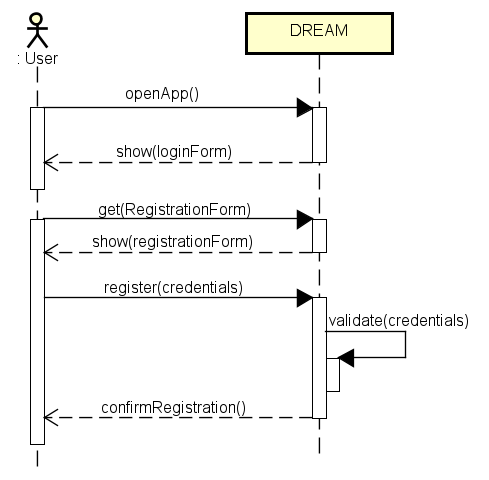
\includegraphics[scale=0.7]{Images/RegistrationSequence.png}
    \caption{Registration sequence diagram}
\end{figure}

\bigskip
\begin{figure}[H]
    \centering
    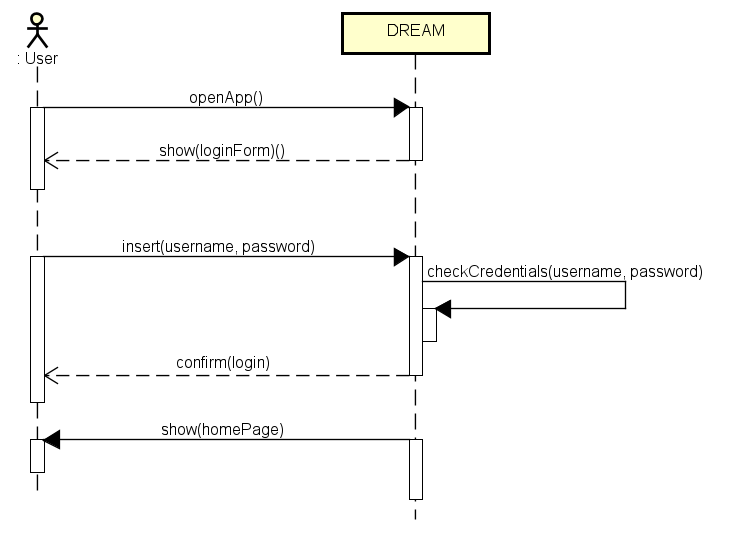
\includegraphics[scale=0.7]{Images/login.png}
    \caption{Log-in sequence diagram}
\end{figure}

\bigskip
\begin{figure}[H]
    \centering
    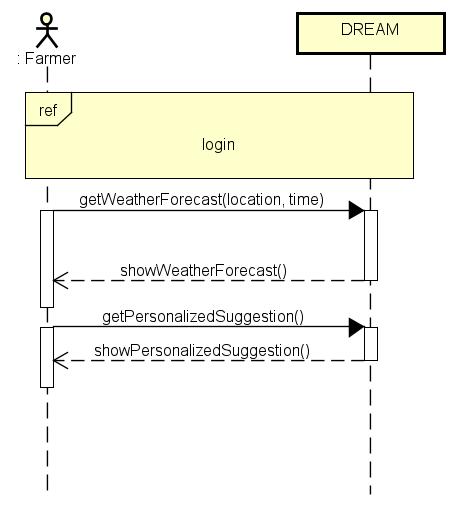
\includegraphics[scale=0.7]{Images/ChecksWeatherForecastSequence.png}
    \caption{Sequence diagram of weather forecast check}
\end{figure}

\bigskip
\begin{figure}[H]
    \centering
    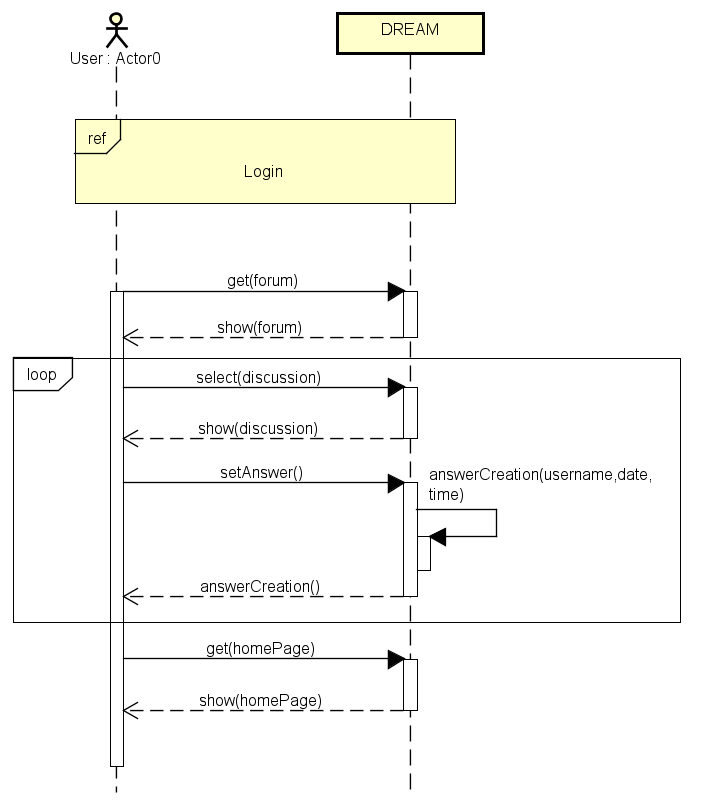
\includegraphics[scale=0.7]{Images/userAnswersForumDiscussion.png}
    \caption{Sequence diagram of users' answer on the forum}
\end{figure}

\bigskip
\begin{figure}[H]
    \centering
    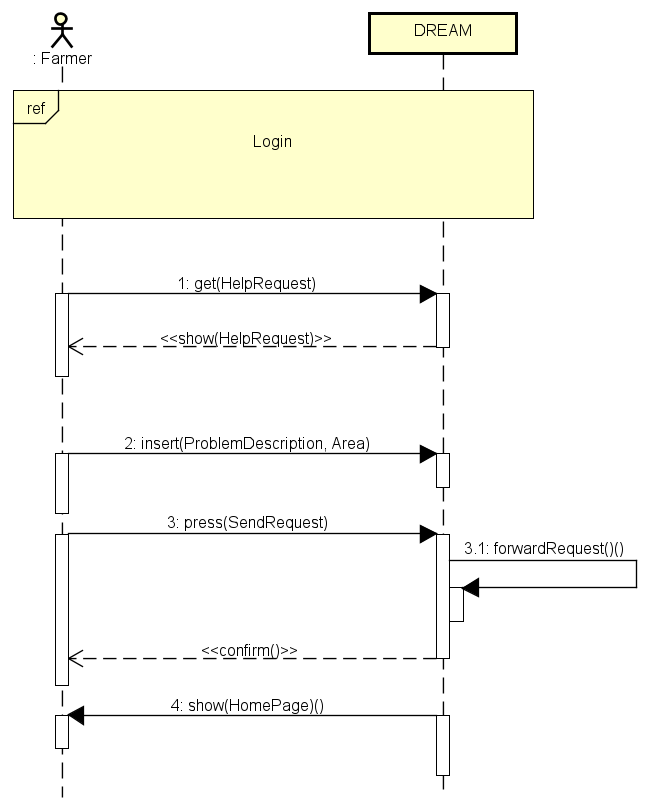
\includegraphics[scale=0.7]{Images/helpRequest.png}
    \caption{Farmer requesting help sequence diagram}
\end{figure}

\bigskip
\begin{figure}[H]
    \centering
    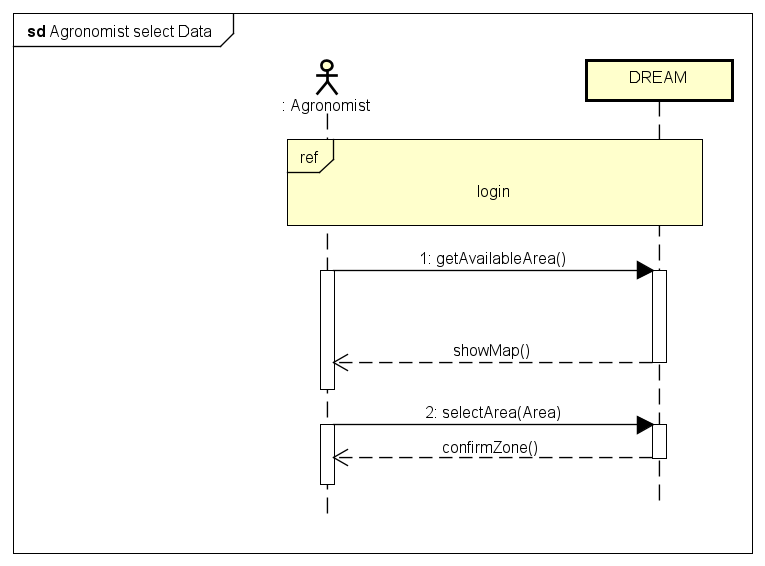
\includegraphics[scale=0.7]{Images/AgronomistSelectDataSequence.png}
    \caption{Sequence diagram of the area selection}
\end{figure}

\bigskip
\begin{figure}[H]
    \centering
    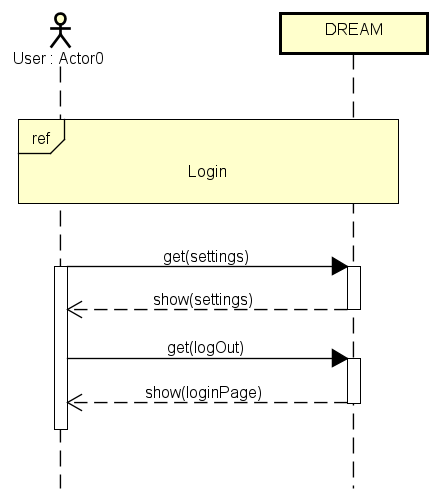
\includegraphics[scale=0.7]{Images/userLogsOut.png}
    \caption{Sequence diagram of log out}
\end{figure}

\bigskip
\begin{figure}[H]
    \centering
    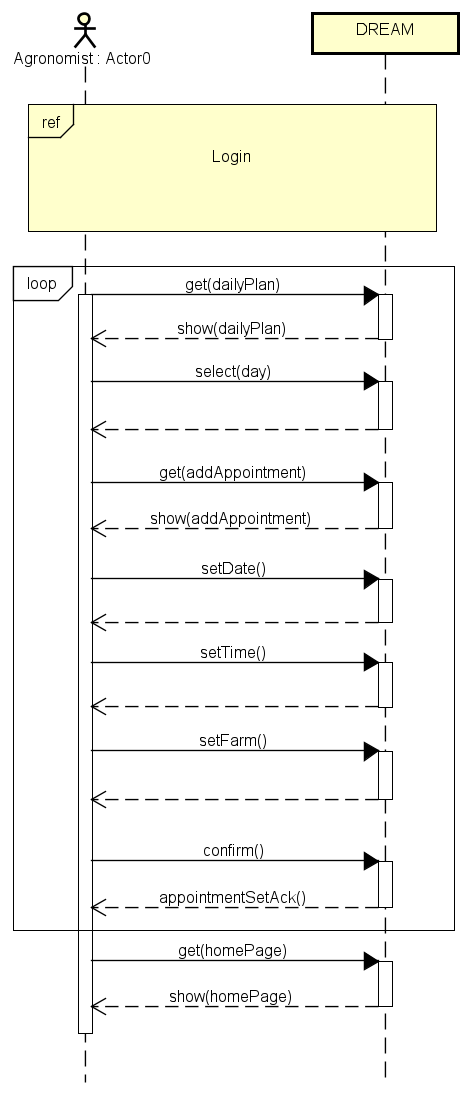
\includegraphics[scale=0.6]{Images/agronomistAddsAppointment.png}
    \caption{Sequence diagram of the addition of an appointment}
\end{figure}

\bigskip
\begin{figure}[H]
    \centering
    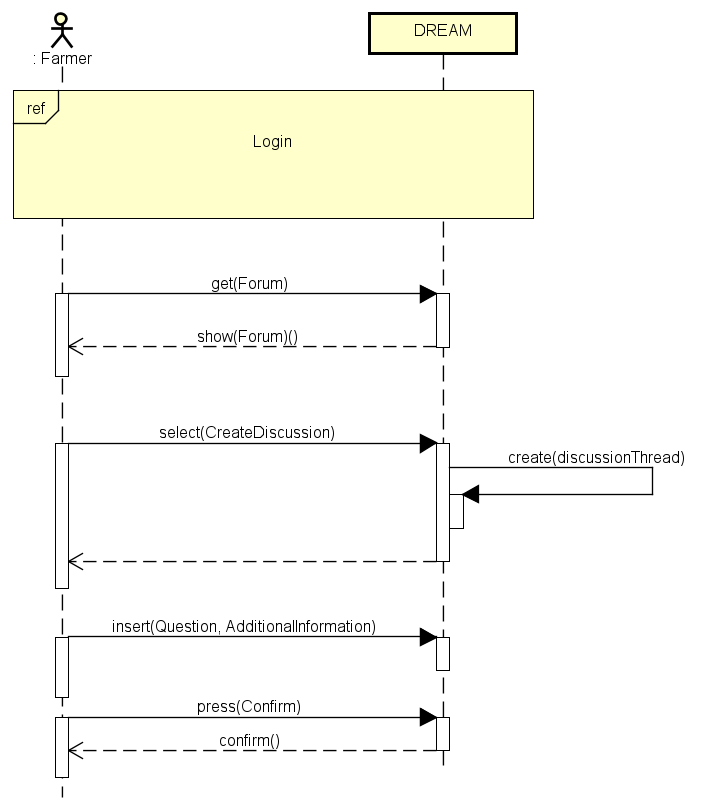
\includegraphics[scale=0.7]{Images/createDiscussion.png}
    \caption{Sequence diagram of the creation of a discussion on the forum}
\end{figure}

\bigskip
\begin{figure}[H]
    \centering
    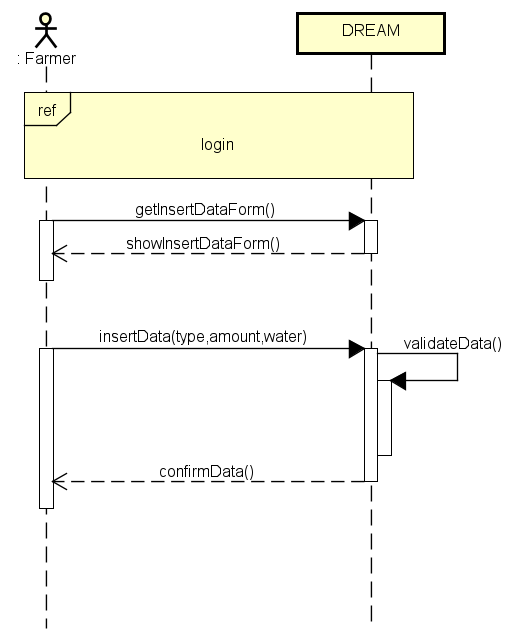
\includegraphics[scale=0.7]{Images/FarmerInsertsDataSequence.png}
    \caption{Farmer insert data concerning production, sequence diagram}
\end{figure}

\bigskip
\begin{figure}[H]
    \centering
    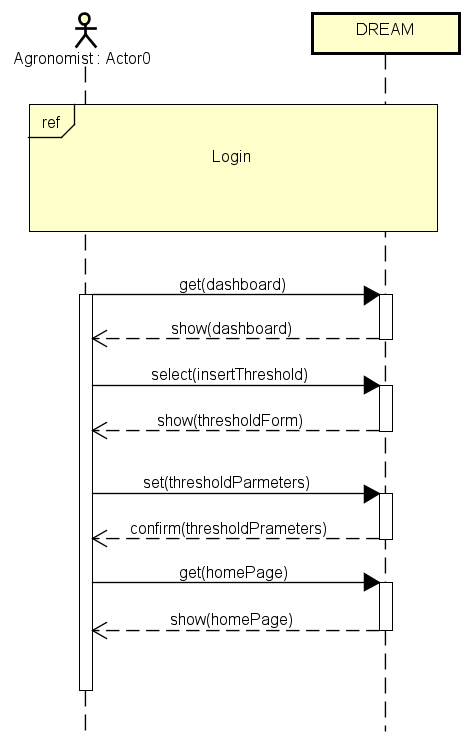
\includegraphics[scale=0.7]{Images/agronomistCreatesThreshold.png}
    \caption{Sequence diagram of threshold creation by an agronomist}
\end{figure}

\bigskip
\begin{figure}[H]
    \centering
    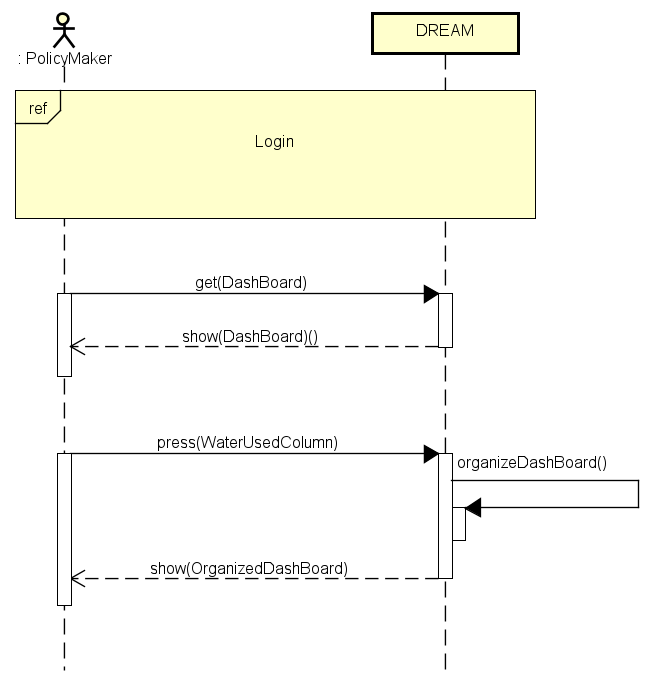
\includegraphics[scale=0.7]{Images/seeDashBoard.png}
    \caption{Sequence diagram of dashboard check by policy maker}
\end{figure}

\bigskip
\begin{figure}[H]
    \centering
    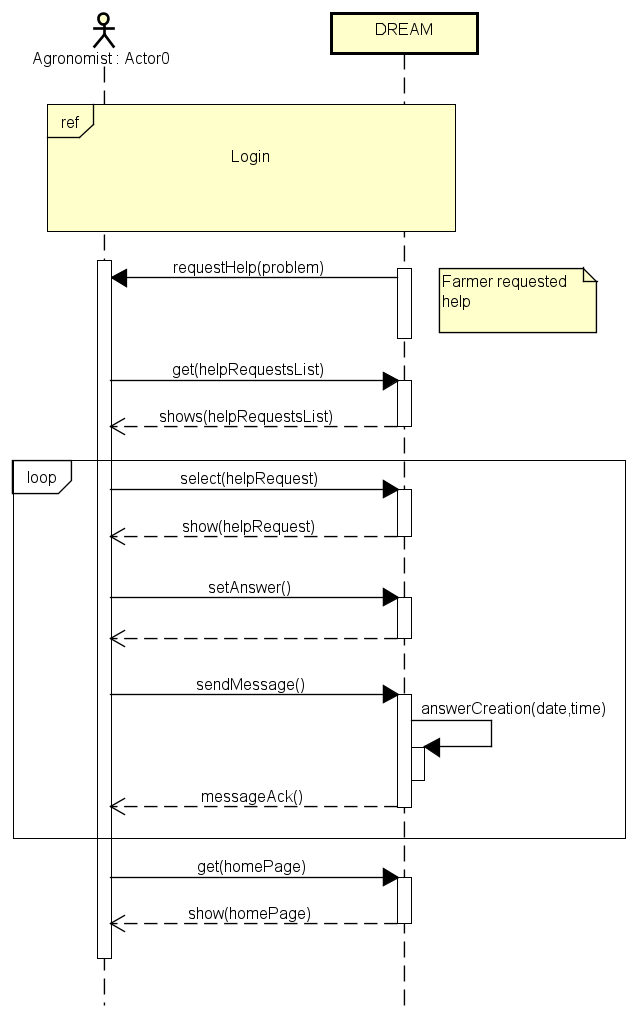
\includegraphics[scale=0.7]{Images/agronomistAnswersHelpRequests.png}
    \caption{Sequence diagram of an agronomist replying to help requests}
\end{figure}

\newpage
\subsection{Performance Requirements}
Though in these cases time is not critical, the requested performances are:
\begin{itemize}
    \item Weather forecasts update must be done within 5 seconds.
    \item When farmer adds production data on the app, the server should be updated within 15 seconds.
    \item When someone answers or requests help on the forum, its post need to be add within 10 seconds.
    \item Daily plan modifications have to be scheduled within 0.5 seconds.
    \item Private help requests and answers, need to be sent to the receiver within 3 seconds.
\end{itemize}


\subsection{Design constraints}
\subsubsection{Hardware limitations}
Running \emph{DREAM} requires a smartphone or computer and a web connection.

\subsection{Software System Attributes}
\subsubsection{Reliability}
\emph{DREAM} should be available 24/7, except for maintenance that has to be performed
only at night and has to last no longer than 2 hours.
\newline The highest number of simultaneous accesses is expected in the harvest time.

\subsubsection{Availability}
The system must be available as much as possible; hence, during daytime is required a minimum value of 97\%.
During the night the availability could be lowered to 95\%.

\subsubsection{Security}
The most critical problems concerning security are privacy, data integrity and authentication. For instance a
MITM attack between policymaker and the server could be dangerous for private data. In order to overcome all
these security problems, the communication between parties should be encrypted through HTTPS protocol.

\subsubsection{Maintainability}
The system must be designed in such a way that permits future addition of functionalities with minimum effort.

\subsubsection{Portability}
\emph{DREAM} should be easily deployable on a dedicated machine, on a virtual private server or on a cloud.
It is in any case usable on every web browser, from every device. The mobile application must be supported by iOS
and Android.

%------------------------------------------------------------------------------------------------------------------------------------------------
\clearpage
{\color{Blue}{\section{Formal Analysis Using Alloy}}}
\label{sect:alloy}
% alloy.sty
% Alloy mode for the LaTeX listings package.
% This is public domain

\lstdefinelanguage{alloy}{
  keywords={%
      assert, pred, all, no, lone, one, some, check, run,
      but, let, implies, not, iff, in, and, or, set, sig, Int, int,
      if, then, else, exactly, disj, fact, fun, module, abstract,
      extends, open, none, univ, iden, seq,
      for, as, sum,
  },
  literate=%
    *{:}{{{\color[HTML]{2835C0}{$\colon$}}}}1
    {>}{{{\color[HTML]{2835C0}{>}}}}1
    {<}{{{\color[HTML]{2835C0}{<}}}}1
    {|}{{{\color[HTML]{2835C0}{|}}}}1
    {==}{{{\color[HTML]{2835C0}{$=$}}}}1
    {=}{{{\color[HTML]{2835C0}{$=$}}}}1
    {!=}{{{\color[HTML]{2835C0}{$\neq$}}}}1
    {&&}{{{\color[HTML]{2835C0}{$\land$}}}}1
    {||}{{{\color[HTML]{2835C0}{$\lor$}}}}1
    {<=}{{{\color[HTML]{2835C0}{$\le$}}}}1
    {>=}{{{\color[HTML]{2835C0}{$\ge$}}}}1
    {!in}{{{\color[HTML]{2835C0}{$\not\in$}}}}1
    {\\in}{{{\color[HTML]{2835C0}{$\in$}}}}1
    {=>}{{{\color[HTML]{2835C0}{$\implies$}}}}2
    % the following isn't actually Alloy, but it gives the option to produce nicer latex
    {|=>}{{{\color[HTML]{2835C0}{$\Rightarrow$}}}}2
    {<=set}{{{\color[HTML]{2835C0}{$\subseteq$}}}}1
    {+set}{{{\color[HTML]{2835C0}{$\cup$}}}}1
    {*set}{{{\color[HTML]{2835C0}{$\cap$}}}}1
    {==>}{{{{\color[HTML]{2835C0}$\Longrightarrow$}}}}3
    {<==>}{$\Longleftrightarrow$}4
    {...}{$\ldots$}1
    {\\hl}{$\hline$}1
    {\\alpha}{$\alpha$}1
    {\\beta}{$\beta$}1
    {\\gamma}{$\gamma$}1
    {\\delta}{$\delta$}1
    {\\epsilon}{$\epsilon$}1
    {\\zeta}{$\zeta$}1
    {\\eta}{$\eta$}1
    {\\theta}{$\theta$}1
    {\\iota}{$\iota$}1
    {\\kappa}{$\kappa$}1
    {\\lambda}{$\lambda$}1
    {\\mu}{$\mu$}1
    {\\nu}{$\nu$}1
    {\\xi}{$\xi$}1
    {\\pi}{$\pi$}1
    {\\rho}{$\rho$}1
    {\\sigma}{$\sigma$}1
    {\\tau}{$\tau$}1
    {\\upsilon}{$\upsilon$}1
    {\\phi}{$\phi$}1
    {\\chi}{$\chi$}1
    {\\psi}{$\psi$}1
    {\\omega}{$\omega$}1
    {\\Gamma}{$\Gamma$}1
    {\\Delta}{$\Delta$}1
    {\\Theta}{$\Theta$}1
    {\\Lambda}{$\Lambda$}1
    {\\Xi}{$\Xi$}1
    {\\Pi}{$\Pi$}1
    {\\Sigma}{$\Sigma$}1
    {\\Upsilon}{$\Upsilon$}1
    {\\Phi}{$\Phi$}1
    {\\Psi}{$\Psi$}1
    {\\Omega}{$\Omega$}1
    {\\EOF}{\;}1
    ,
  sensitive=true,  % case sensitive
  morecomment=[l]//,%
  morecomment=[l]{--},%
  morecomment=[s]{/*}{*/},%
  morestring=[b]",
  numbers=none,
  firstnumber=1,
  numberstyle=\tiny,
  stepnumber=2,
  basicstyle=\scriptsize\ttfamily,
  commentstyle=\color[HTML]{00A108}\itshape,
  keywordstyle=\color[HTML]{2835C0}\bfseries,
  ndkeywordstyle=\bfseries,
}

% inline
\def\A{%
    \lstinline[language=alloy,basicstyle=\ttfamily,columns=fixed]}

% paragraph
\lstnewenvironment{alloy}[1][]{%
  \lstset{language=alloy,
    floatplacement={tbp},captionpos=b,
    xleftmargin=8pt,xrightmargin=8pt,basicstyle=\ttfamily,#1}}{}

% paragraph from file
\newcommand{\alloyfile}[1]{
  \lstinputlisting[language=alloy,%
    frame=lines,xleftmargin=8pt,xrightmargin=8pt,basicstyle=\ttfamily,columns=fixed]{#1}
}

\lstset{
    %Add this if you want to display border around your code  
    %frame=single,
    breaklines=true,
    postbreak=\raisebox{0ex}[0ex][0ex]{\ensuremath{\color{red}\hookrightarrow\space}}
}

%------------------------------------------------------------------------------------------------------------------------------------------------
\clearpage
{\color{Blue}{\section{Effort Spent}}}
\label{sect:effort}
\begin{table}[H]
    \centering
    \begin{tabular}{|l|l|l|}
        \multicolumn{3}{c}{\textbf{Lorenzo Iovine}}                   \\
        \hline
        \textbf{Date} & \textbf{Hours} & \textbf{Description}          \\\hline
        2021-11-29    & 7h             & Introduction, Purpose, Scope \& Goals                  \\\hline
        2021-11-30    & 5h             & UML diagram, statecharts \& World and the Machine      \\\hline
        2021-12-01    & 7h             & Product functions                                      \\\hline
        2021-12-02    & 3h             & Product functions, User characteristics \& Assumptions \\\hline
        2021-12-02    & 4h             & Mockups                                                \\\hline
        2021-12-03    & 4h             & Use cases                                              \\\hline
        2021-12-04    & 2h             & Use cases                                              \\\hline
        2021-12-04    & 4h             & Sequence diagram                                       \\\hline
        2021-12-05    & 3h             & Review                                                 \\\hline
        2021-12-06    & 5h             & Review \& Alloy                                        \\\hline
        2021-12-07    & 3h             & Alloy                                                  \\\hline\hline
                      & 47h            &                                                        \\\hline
    \end{tabular}
\end{table}
\begin{table}[H]
    \centering
    \begin{tabular}{|l|l|l|}
        \multicolumn{3}{c}{\textbf{Nicola Landini}}                      \\
        \hline
        \textbf{Date} & \textbf{Hours} & \textbf{Description}                                   \\\hline
        2021-11-29    & 7h             & Introduction, Purpose, Scope \& Goals                  \\\hline
        2021-11-30    & 5h             & UML diagram, statecharts \& World and the Machine      \\\hline
        2021-12-01    & 7h             & Product functions                                      \\\hline
        2021-12-02    & 3h             & Product functions, User characteristics \& Assumptions \\\hline
        2021-12-02    & 4h             & Mockups                                                \\\hline
        2021-12-03    & 4h             & Customer Interfaces                                    \\\hline
        2021-12-04    & 2h             & Customer Interfaces                                    \\\hline
        2021-12-04    & 4h             & Sequence diagram                                       \\\hline
        2021-12-05    & 3h             & Review                                                 \\\hline
        2021-12-06    & 5h             & Review \& Alloy                                        \\\hline
        2021-12-07    & 3h             & Alloy                                                  \\\hline\hline
                      & 47h            &                                                        \\\hline
    \end{tabular}
\end{table}
\begin{table}[H]
    \centering
    \begin{tabular}{|l|l|l|}
        \multicolumn{3}{c}{\textbf{Francesco Leone}}                      \\
        \hline
        \textbf{Date} & \textbf{Hours} & \textbf{Description}              \\\hline
        2021-11-29    & 7h             & Introduction, Purpose, Scope \& Goals                  \\\hline
        2021-11-30    & 5h             & UML diagram, statecharts \& World and the Machine      \\\hline
        2021-12-01    & 7h             & Product functions                                      \\\hline
        2021-12-02    & 3h             & Product functions, User characteristics \& Assumptions \\\hline
        2021-12-02    & 4h             & Requirements                                           \\\hline
        2021-12-03    & 4h             & Use cases                                              \\\hline
        2021-12-04    & 2h             & Use cases                                              \\\hline
        2021-12-04    & 4h             & Sequence diagram                                       \\\hline
        2021-12-05    & 3h             & Review                                                 \\\hline
        2021-12-06    & 5h             & Review \& Alloy                                        \\\hline
        2021-12-07    & 3h             & Alloy                                                  \\\hline\hline
                      & 47h            &                                                        \\\hline
    \end{tabular}
\end{table}

%------------------------------------------------------------------------------------------------------------------------------------------------




\end{document}
